\documentclass[10pt,a4paper]{article}

%%%%%%%%%%%%%%%%%%%%%%%%%%%
% MODIFY:

\newcommand{\authorA}{Ahmad Bin Qasim (03693345)}
\newcommand{\authorB}{Kaan Atukalp (03709123)}
\newcommand{\authorC}{Martin Meinel (03710370)}
\newcommand{\groupNumber}{H} % - YOUR GROUP NUMBER
\newcommand{\exerciseNumber}{4} % - THE NUMBER OF THE EXERCISE
\newcommand{\sourceCodeLink}{https://gitlab.lrz.de/ga53rog/praktikum-ml-crowd}

\newcommand{\workPerAuthor}{
\authorA&Task 1&33\%\\
      &Task 2&33\%\\
      &Task 3&33\%\\
      &Task 4&33\%\\
      &Task 5&33\%\\
      \hline
\authorB&Task 1&33\%\\
      &Task 2&33\%\\
      &Task 3&33\%\\
      &Task 4&33\%\\
      &Task 5&33\%\\
      \hline
\authorC&Task 1&33\%\\
      &Task 2&33\%\\
      &Task 3&33\%\\
      &Task 4&33\%\\
      &Task 5&33\%\\
}

%%%%%%%%%%%%%%%%%%%%%%%%%%%

%%
% imports for the exercise sheets
%

\usepackage[utf8]{inputenc}
\usepackage{amsmath}
\usepackage{amsfonts}
\usepackage{amssymb}

\usepackage[yyyymmdd]{datetime}
\renewcommand{\dateseparator}{--}

\usepackage[left=2cm,right=2cm,top=3cm,bottom=3cm]{geometry}

\usepackage{hyperref}

\usepackage{amsthm}
\newtheorem{lem}{Lemma}
\newtheorem{thm}{Theorem}
\newtheorem{cor}{Corollary}
\newtheorem{rem}{Remark}
\newtheorem{definition}{Definition}
\newtheorem{ter}{Terminology}

\usepackage{graphicx}

\newcommand{\M}{\mathcal{M}}
\newcommand{\N}{\mathcal{N}}
\newcommand{\K}{\mathcal{K}}
\newcommand{\SPDk}{\mathbb{P}^k}
\newcommand{\vol}{\text{vol}}

\newcommand{\Figref}[1]{Figure~\ref{#1}}
\newcommand{\figref}[1]{figure~\ref{#1}}
\newcommand{\Eqnref}[1]{Equation~(\eqref{#1})}
\newcommand{\eqnref}[1]{equation~(\eqref{#1})}

\usepackage{float}
\usepackage{tabularx}
\usepackage{subcaption}
\usepackage{mwe}

\usepackage{fancyhdr}
\pagestyle{fancy}

\usepackage{totcount}
\newtotcounter{taskCounter}
\newtotcounter{pointCounter}
\newenvironment{task}[1]{\noindent\stepcounter{taskCounter}\textbf{Report on task #1}\smallbreak\hrule\smallbreak}{\smallbreak\hrule\bigbreak}


\title{Report for exercise \exerciseNumber~from group~\groupNumber}

\makeatletter
\let\thetitle\@title
\let\theauthor\@author
\let\thedate\@date
\makeatother

\providecommand{\versiondate}{\today}

\lhead{Exercise sheet \exerciseNumber}
\chead{Master Praktikum: Modelling and Simulation of Crowds WS2019/20}
\rhead{TUM}
\lfoot{Report of Group \groupNumber}
\cfoot{\thepage}
\rfoot{Last compiled: \versiondate}
\renewcommand{\headrulewidth}{0.4pt}
\renewcommand{\footrulewidth}{0.4pt}

\newcommand{\frontpage}{
\begin{center}
\textbf{\thetitle}\\~\\
\end{center}
\begin{table}[H]
\begin{tabular}{ll}
Tasks addressed:&\total{taskCounter}\\
Authors:&\authorA\\
&\authorB\\
&\authorC\\
Last compiled:&\versiondate\\
Source code:&\sourceCodeLink
\end{tabular}
\end{table}
\vfill
The work on tasks was divided in the following way:
\begin{table}[H]
\begin{tabularx}{\textwidth}{X|p{2cm}|p{2cm}}
\workPerAuthor
\end{tabularx}
\end{table}
\newpage
}

\begin{document}

\frontpage

\begin{task}{1, Principal component analysis}
First part: We used the data set from moodle and applied Principal Component Analysis. In Figure \ref{fig:task1_part1} you can see the original data set with the two principal components marked in red. The first principal component is the one pointing to the right upper corner. So the second one is the other principal component pointing towards the left upper corner and being orthogonal to the first principal component.
\begin{figure}[H]
\centering
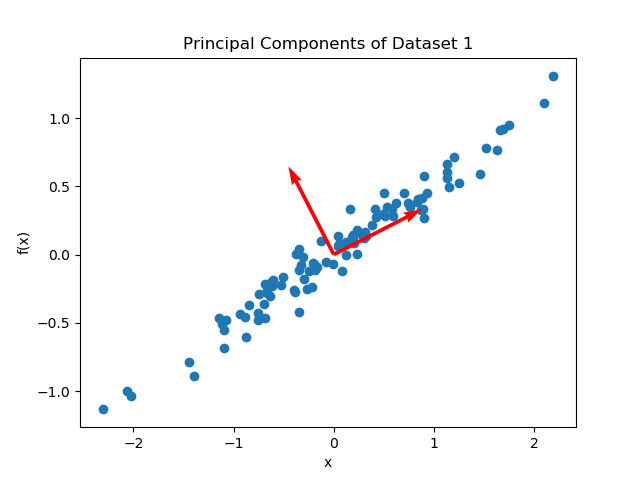
\includegraphics[width=0.7\textwidth]{../plots/task1/PCA_1.png}
\caption{Plot of the data set with the two first principal components}
\label{fig:task1_part1}
\end{figure}
The energy of a principal component describes how much variance of the data the principal component covers. In the following table you can see the energy of the drawn two principal components and the sum of them. It can be seen that the first principal component has a big energy value and therefore covers almost all the variance of the data. From the sum of both energy values it can be seen that both principal components cover the entire data set.
\begin{center}
\begin{tabular}{l|c}
&Energy \\
\hline
Principal Component 1& 0.993\\
Principal Component 2& 0.07\\
First two components & 1.00\\
\hline
\end{tabular}
\end{center}
\bigbreak
Second Part: 
At first we used the rows of the images as single data points, but after seeing the reconstructed images, we considered the columns of the image as single data points and the resulting reconstructed pictures were reconstructed much better than before. Figure \ref{fig:task1_part2} shows all the four reconstructed images starting with using all principal components to only using the first ten principal components.
\begin{figure}[H]
\centering
\begin{subfigure}[b]{0.475\textwidth}
\centering
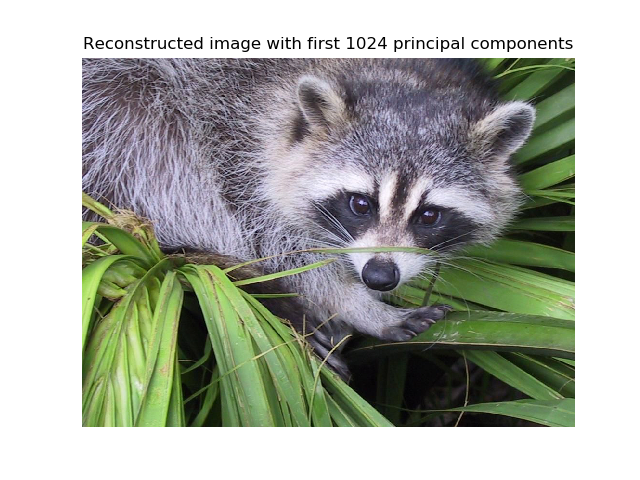
\includegraphics[width=\textwidth]{../plots/task1/task1_2_firstall.png}
\caption[]
{{\small Reconstructed image of a raccoon using all principal components}}
\label{fig:task1_part2_all}
\end{subfigure}
\hfill
\begin{subfigure}[b]{0.475\textwidth}
\centering
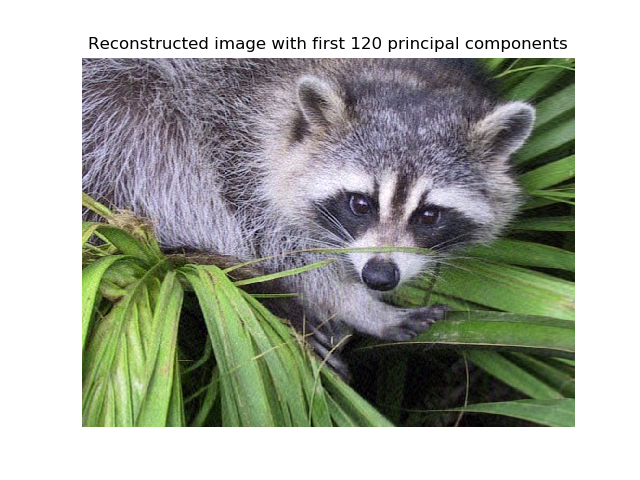
\includegraphics[width=\textwidth]{../plots/task1/task1_2_first120.png}
\caption[]
{{\small Reconstructed image of a raccoon using the first 120 principal components}}
\label{fig:task1_part2_120}
\end{subfigure}
\hfill
\vskip\baselineskip
\begin{subfigure}[b]{0.475\textwidth}
\centering
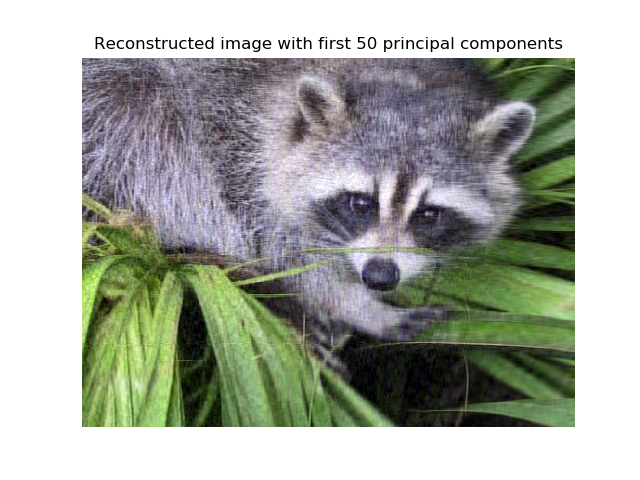
\includegraphics[width=\textwidth]{../plots/task1/task1_2_first50.png}
\caption[]
{{\small Reconstructed image of a raccoon using the first 50 principal components}}
\label{fig:task1_part2_50}
\end{subfigure}
\quad
\begin{subfigure}[b]{0.475\textwidth}
\centering
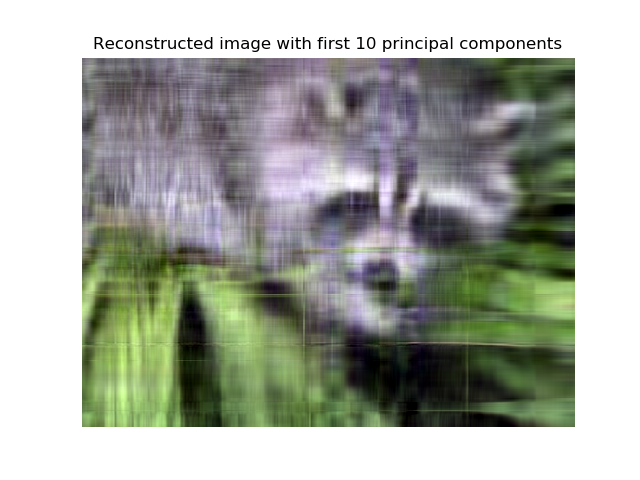
\includegraphics[width=\textwidth]{../plots/task1/task1_2_first10.png}
\caption[]
{{\small Reconstructed image of a raccoon using the first 10 principal components}}
\label{fig:task1_part2_10}
\end{subfigure}
\caption{The reconstructed images of a raccoon using different numbers of principal components}
\label{fig:task1_part2}
\end{figure}
It can be seen that the reconstructed images using the first 120 or first 50 are close to the original picture. The reconstructed image where only the first 10 principal components are used seems blurry but the image can still be recognized. By using the first 20 out of 1023 principal components, we can cover 99.01\% of the variance.
\bigbreak
Third Part: We have a data file containing the (x,y) positions for 15 pedestrians over 1000 time steps. Figure \ref{fig:task1_part3_1} visualizes the path from the first two pedestrians in space. It shows that the first two pedestrians are walking in loops.
\begin{figure}[H]
\centering
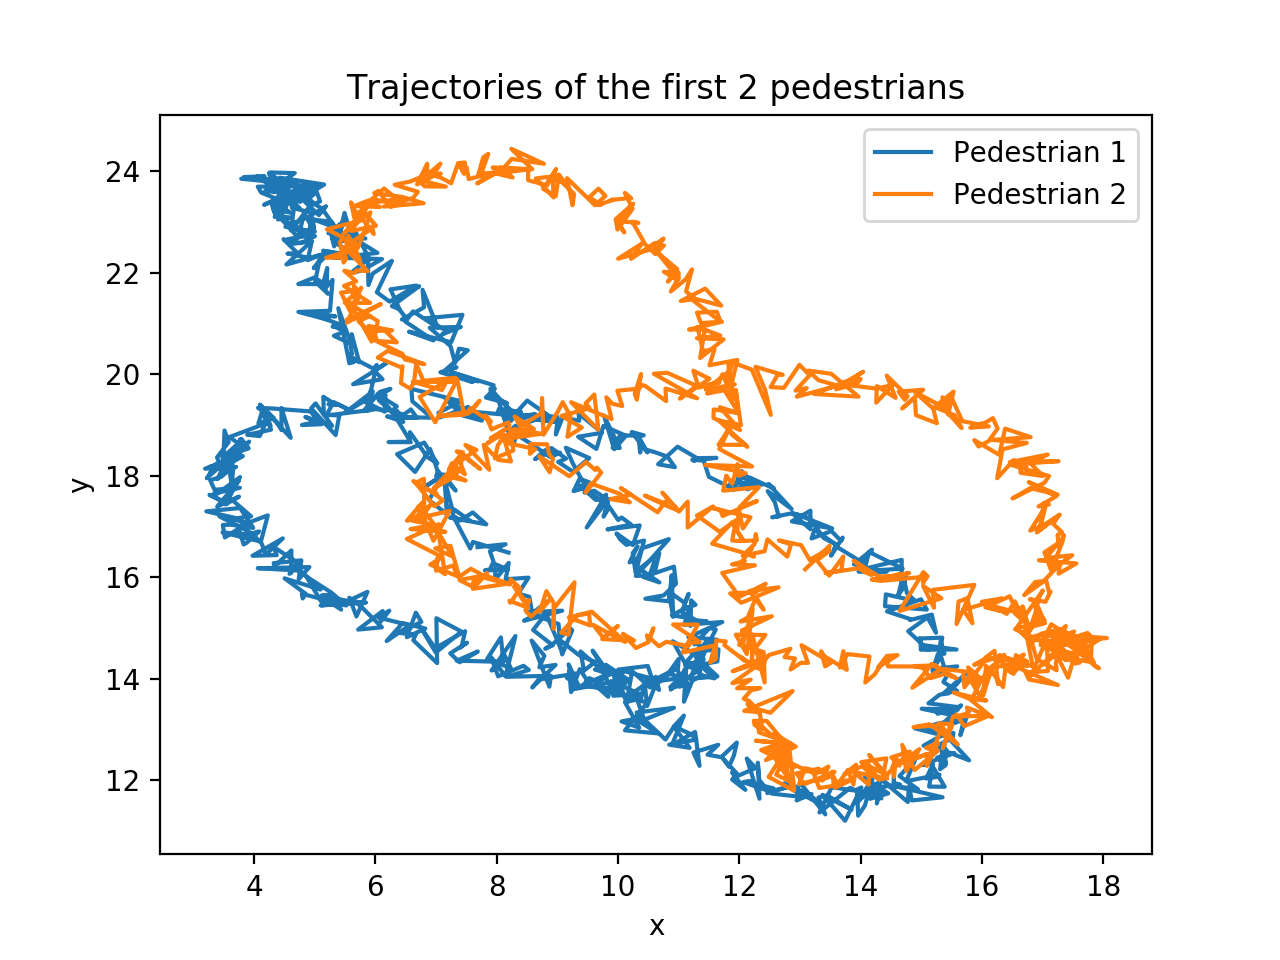
\includegraphics[width=0.7\textwidth]{../plots/task1/task1_3.png}
\caption{Visualized paths for the first two pedestrians over 1000 time steps}
\label{fig:task1_part3_1}
\end{figure}
Now we use Principal Component Analysis and use the first two principal components of it to project the 30-dimensional data points to the first two principal components. The following table shows the energy values for the  first two principal components and shows that the first two principal components cover a variance of almost 85\% of the data.
\begin{center}
\begin{tabular}{l|c}
& energy\\
\hline
Principal Component 1& 0.473\\
Principal Component 2& 0.376\\
First two  principal components together&0.849\\
\hline
\end{tabular}
\end{center}
We tried to reconstruct the original trajectories from Figure \ref{fig:task1_part3_1} with the first two principal components.
The following Figure \ref{fig:task1_part3_2} shows the reconstructed trajectories for the first two pedestrians using the first two principal components.
\begin{figure}[H]
\centering
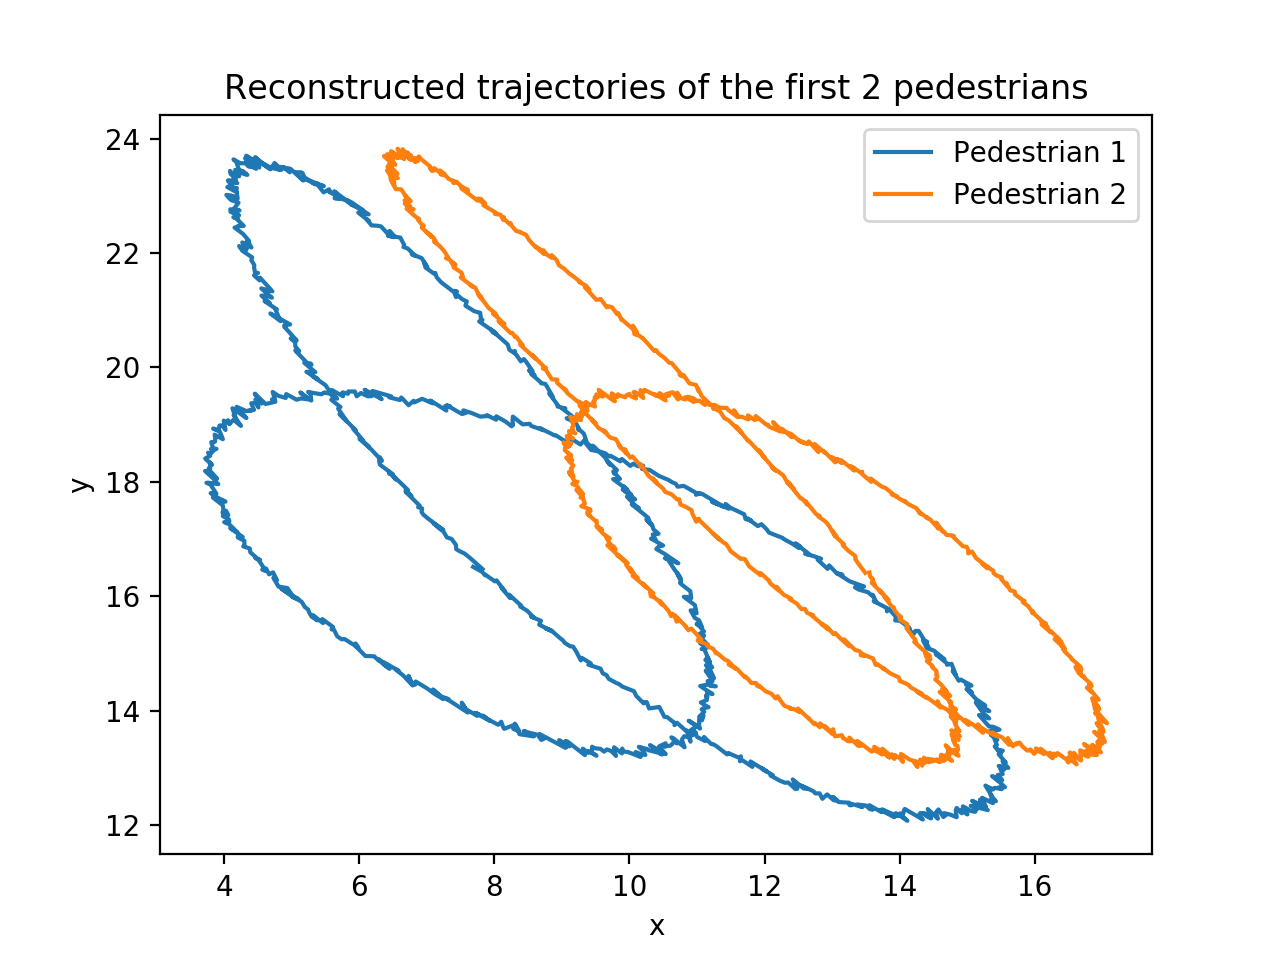
\includegraphics[width=0.7\textwidth]{../plots/task1/Task1_3reconstructed.png}
\caption{Reconstructed trajectories from using the first two principal components}
\label{fig:task1_part3_2}
\end{figure}
From comparing the trajectories of the first two pedestrians from Figure \ref{fig:task1_part3_1} to Figure \ref{fig:task1_part3_2} it can be seen that the trajectories are similar. Besides of that, the total amount of energy is almost 85\% and this is why in our opinion the first two principal components are enough to capture most of the energy.
\bigbreak
It took us two days to implement and test the implementation of task1. \\
We could represent the data very accurately. Especially for part 2 of task 1, it can be seen that even the first 50 principal component are sufficient to visualize the picture of the raccoon. We measured the accuracy by using the energy, which describes how much variance of the original data can be described by using the corresponding principal component. Besides of that, we generated the reconstructed images and compared them to the original image. \\
Principal Component Analysis is used for image compression. It was interesting to see how well it works and we learned that the result is different if you consider the rows or the columns of an image as single data points. So we learned that it makes sense to think about how to apply Principal Component Analysis to the data in advance. Furthermore we learned that often the first few principal components are sufficient to cover the data. \\
\end{task}
\begin{task}{2, Diffusion Maps}
First Part: Five eigenfunctions of the given periodic data set were computed using Diffusion Maps. As seen in Figure \ref{fig:task2_part1}, the eigenfunctions have mapped the data on scaled sine/cosine waves with varying periods.

\begin{figure}[H]
\centering
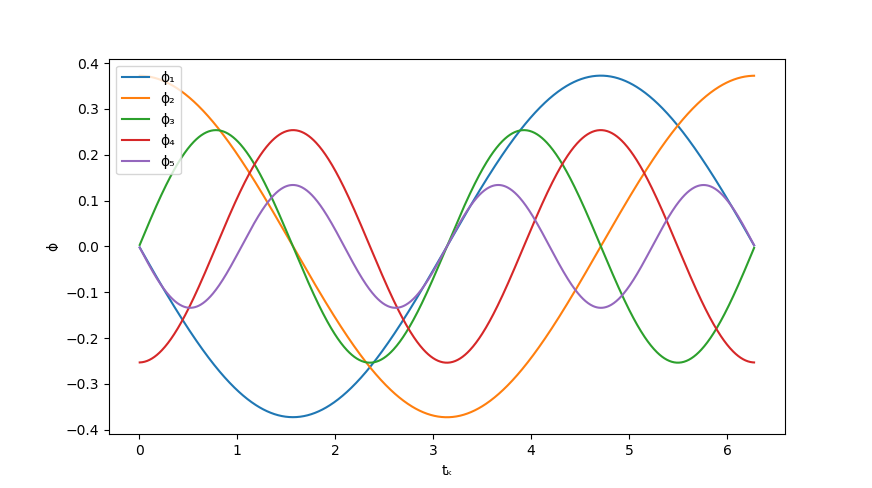
\includegraphics[width=0.7\textwidth]{../plots/task2/task2_1.png}
\caption{Values of the eigenfunctions with respect to the t value.}
\label{fig:task2_part1}
\end{figure}

\bigbreak
Second Part: 
Starting from $l=5$, the eigenfunctions $\phi_l$ are not a function of $\phi_1$ anymore. This can be seen in Figure \ref{fig:task2_part2} where the eigenfunctions for $l=2, 3, 4$ could easily be represented with commonly known polynomial or trigonometric functions, whereas the others show no relevant correlation for all values of $\phi_1$. \\

\begin{figure}[H]
\centering
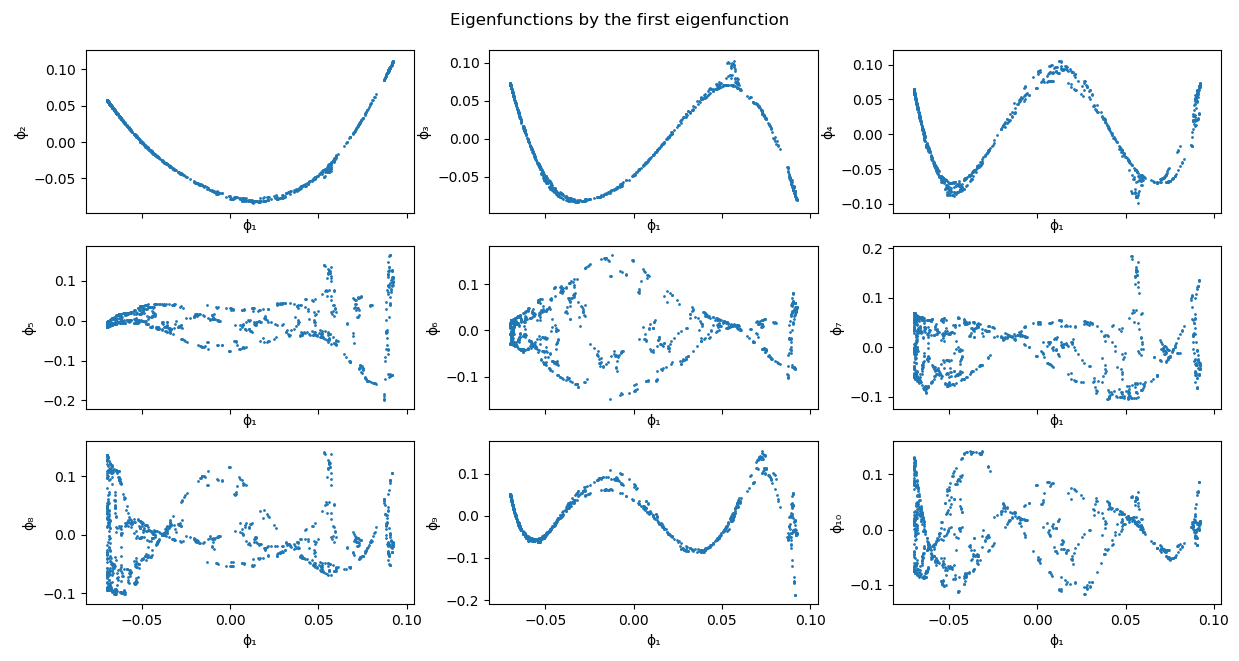
\includegraphics[width=0.7\textwidth]{../plots/task2/task2_2.png}
\caption{Values of eigenfunctions for $l=2, 3, 4, 5, 6, 7, 8, 9, 10$ with respect to $\phi_1$.}
\label{fig:task2_part2}
\end{figure}

When PCA is applied to the data set, the resulting energy values for the first 3 principal components are as follows: \\

\begin{center}
\begin{tabular}{l|c}
& energy\\
\hline
Principal Component 1& 0.38\\
Principal Component 2& 0.33\\
Principal Component 3& 0.29\\
\hline
\end{tabular}
\end{center}

The first two principal components cover only 72\% of the data, so we would lose 29\% of the data. Thus, it makes more sense to take all principal components instead of the first two. 

\bigbreak
Third Part:
By plotting the eigenfunctions in a 3D plot as seen in Figure \ref{fig:task2_part3}, it can be seen that the first two eigenfunctions are enough to capture all the data. Not a single pair of points seems to have the same value (colour) pair in the first 2 eigenfunctions, which can be seen when the Figures \ref{fig:task2_part3_1} and \ref{fig:task2_part3_2} are compared side by side.\\

\begin{figure}[H]
\centering
\begin{subfigure}[b]{0.475\textwidth}
\centering
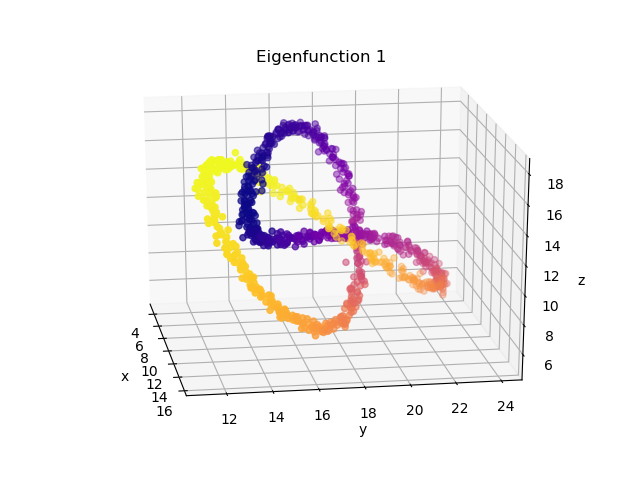
\includegraphics[width=\textwidth]{../plots/task1/task2_3_eigenfunction1.png}
\caption[]{{\small Values assigned by the first eigenfunction}}
\label{fig:task2_part3_1}
\end{subfigure}
\hfill
\begin{subfigure}[b]{0.475\textwidth}
\centering
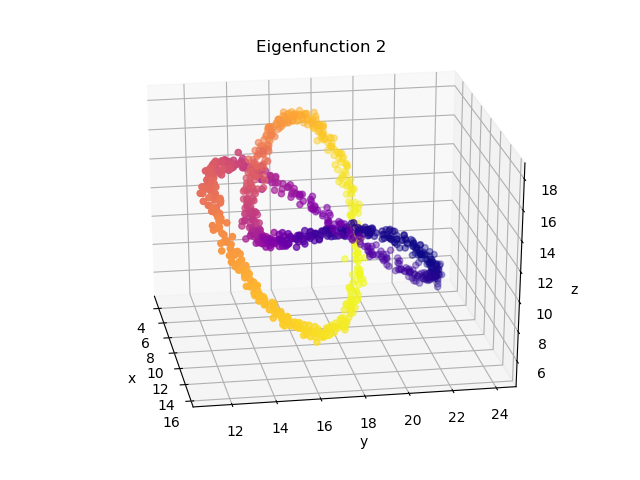
\includegraphics[width=\textwidth]{../plots/task1/task2_3_eigenfunction2.png}
\caption[]{{\small Values assigned by the second eigenfunction}}
\label{fig:task2_part3_2}
\end{subfigure}
\hfill
\vskip\baselineskip
\begin{subfigure}[b]{0.475\textwidth}
\centering
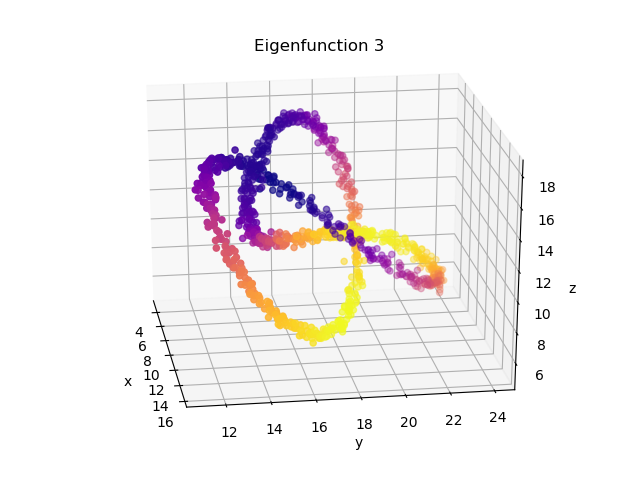
\includegraphics[width=\textwidth]{../plots/task1/task2_3_eigenfunction3.png}
\caption[]{{\small Values assigned by the third eigenfunction}}
\label{fig:task2_part3_3}
\end{subfigure}
\quad
\caption{Graphs showing the values assigned for the first three eigenfunctions. Brighter colour indicates a higher real number.}
\label{fig:task2_part3}
\end{figure}

\end{task}

\begin{task}{3, Training a Variational Autoencoder on MNIST}
\begin{enumerate}
	\item We used a linear activation function to approximate the mean and standard deviation of the posterior distribution because, the mean and standard deviation values are unbounded. Other activation functions bound the output value to a certain range. We considered different activation functions but discarded it because of the bounded output. [\ref{tab:activation}]
\begin {table}[H]
\caption {Different activation functions} \label{tab:activation} 
\begin{center}
\begin{tabular}{ | m{10em} | m{10em}| } 
\hline
Activation Function& Bounds \\ 
\hline \hline
Sigmoid & (0,1) \\ 
\hline
Tanh & (-1,1) \\
\hline
Relu & max(0,x) \\
\hline
\end{tabular}
\end{center}
\end{table}
	\item If the reconstructed image are much better then the generated images then, it means that the model has been overfitted to the input data distribution. This can happen when the KL-divergence loss (latent loss) of the approximated posterior distribution does not converge while the reconstruction loss of the input distribution converges. 
	
	In order to solve this problem, the reconstruction loss and the KL-divergence loss can be weighted to give more weight to the latter.
	
	\item After training the Variational Autoencoder model, We plotted the desired graphs. The latent space of the encoder is 2 dimensional. [\ref{fig:latent-2}]. In addition to the configurations provided in the exercise sheet, related to the model, the following changes were made:
	\begin{itemize}
		\item The output of the decoder is not the mean of likelihood but the predicted data points. This modification within the decoder can be considered as probabilistic as well because it is equivalent to modeling likelihood as Gaussian with identity covariance
		\item Binary cross entropy is used to calculated the reconstruction loss with the predicted data points from decoder and the input data as the target.
		\item The last layer of decoder uses a Sigmoid activation as the data in mnist is grayscale. 
	\end{itemize}
	
\begin{figure}[H]
\caption{results obtained with a 2 dimensional latent space}
\label{fig:latent-2} 
\begin{tabular}{cccc}
  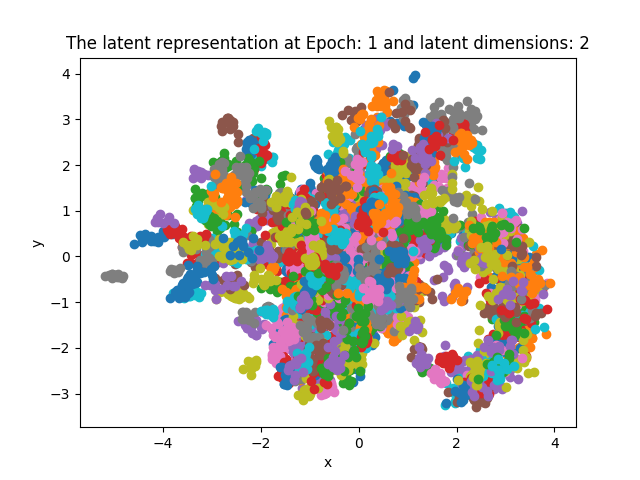
\includegraphics[width=0.23\textwidth]{../plots/task3/latent_epoch1_latent2.png} &   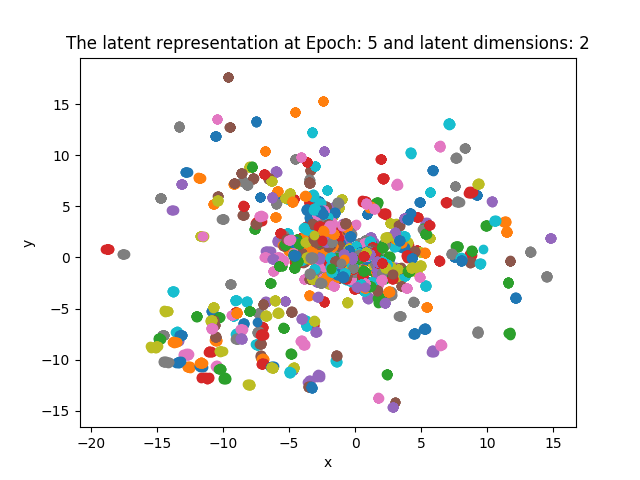
\includegraphics[width=0.23\textwidth]{../plots/task3/latent_epoch5_latent2.png} & 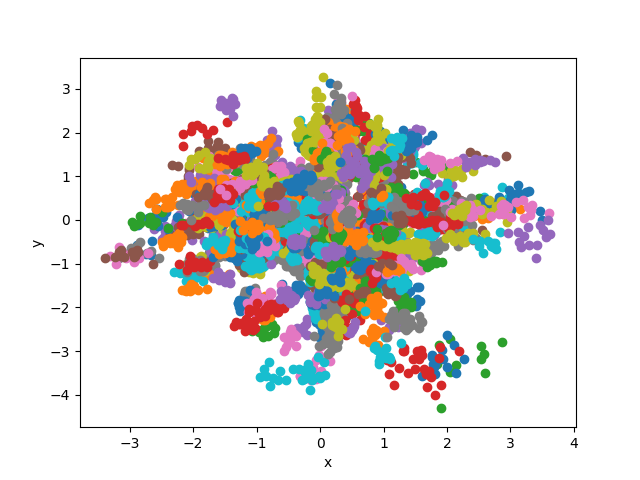
\includegraphics[width=0.23\textwidth]{../plots/task3/latent_epoch25_latent2.png} &   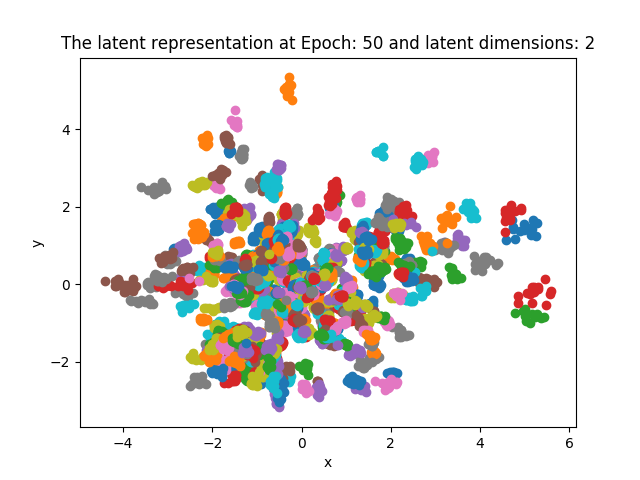
\includegraphics[width=0.23\textwidth]{../plots/task3/latent_epoch50_latent2.png} \\
      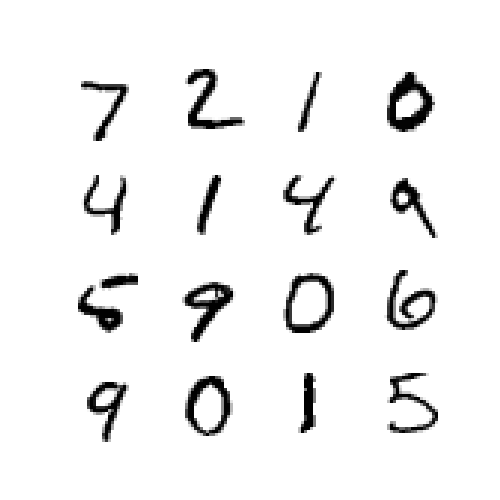
\includegraphics[width=0.23\textwidth]{../plots/task3/real_epochs1_latent2.png} &   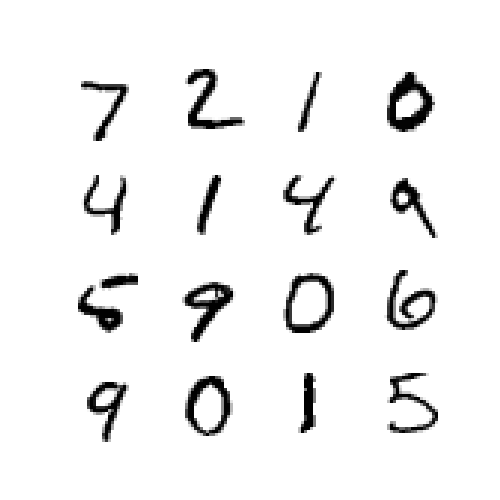
\includegraphics[width=0.23\textwidth]{../plots/task3/real_epochs5_latent2.png} & 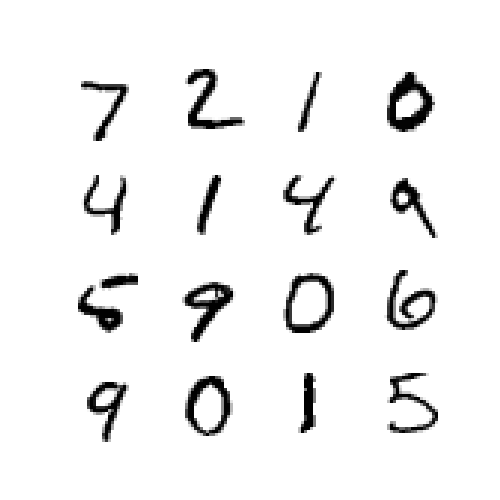
\includegraphics[width=0.23\textwidth]{../plots/task3/real_epochs25_latent2.png} &   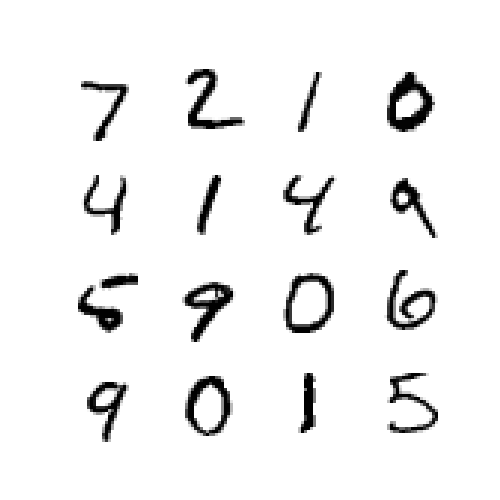
\includegraphics[width=0.23\textwidth]{../plots/task3/real_epochs50_latent2.png} \\
    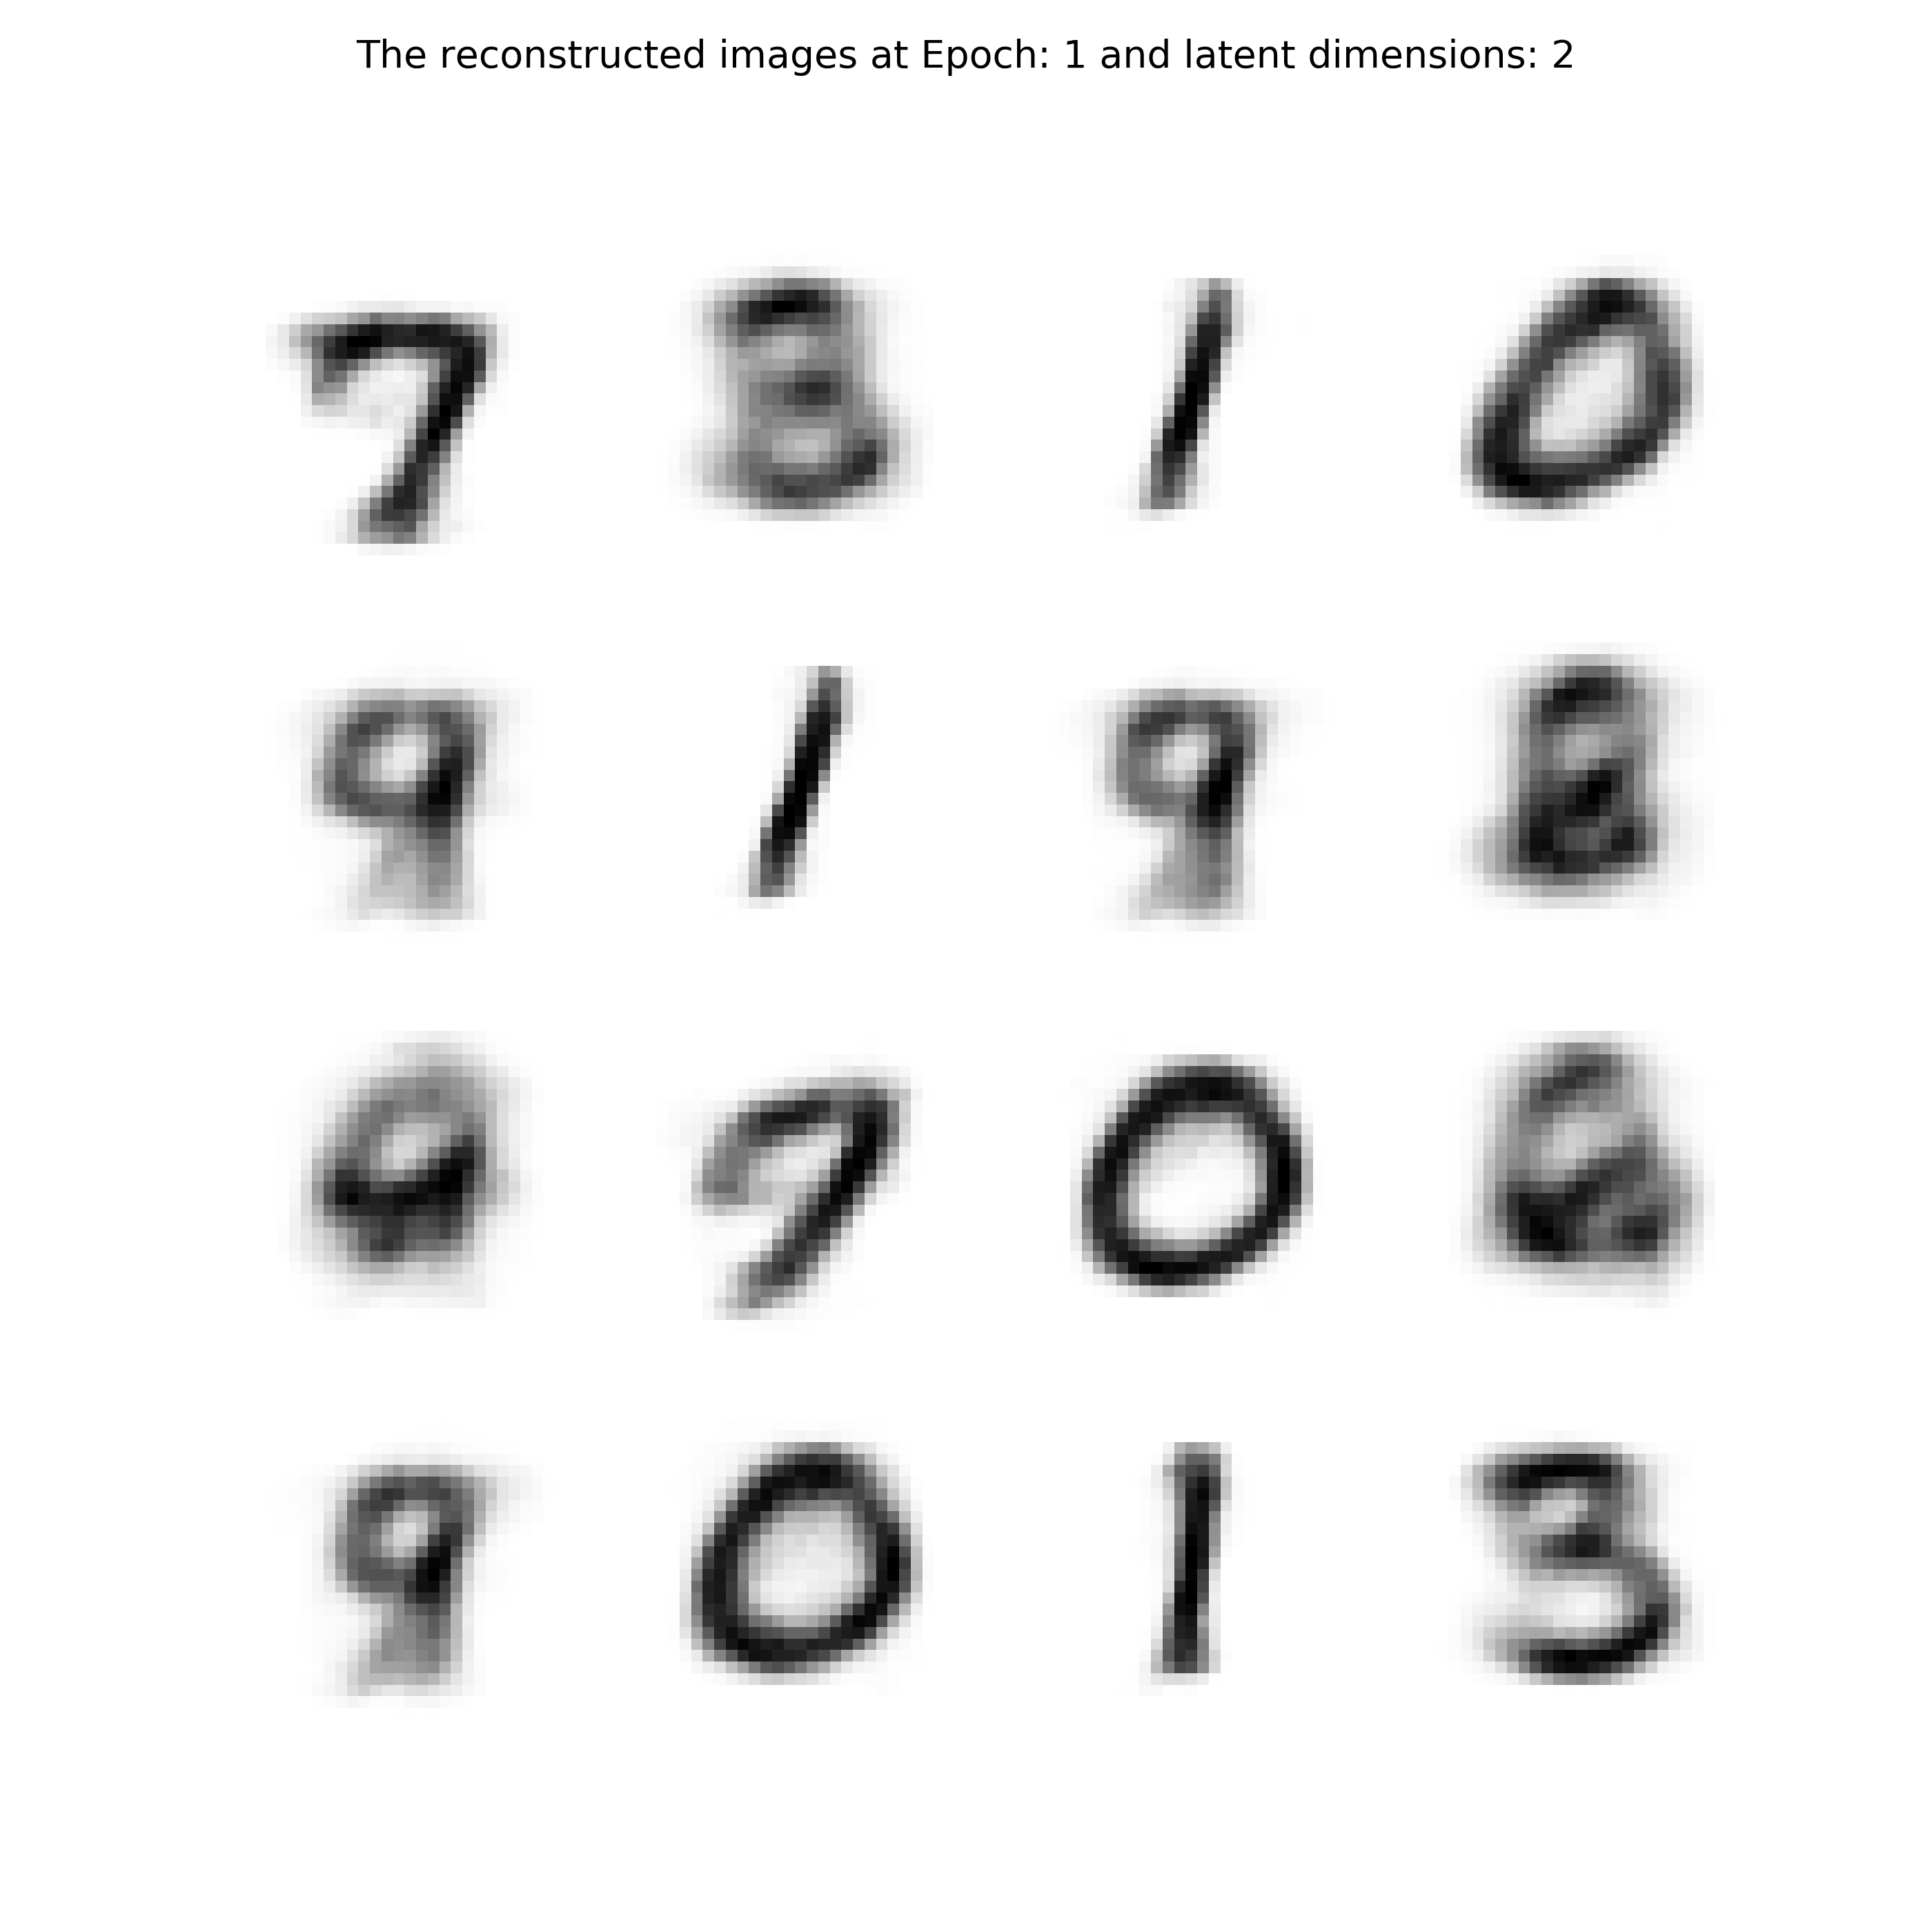
\includegraphics[width=0.23\textwidth]{../plots/task3/reconstructed_epochs1_latent2.png} &   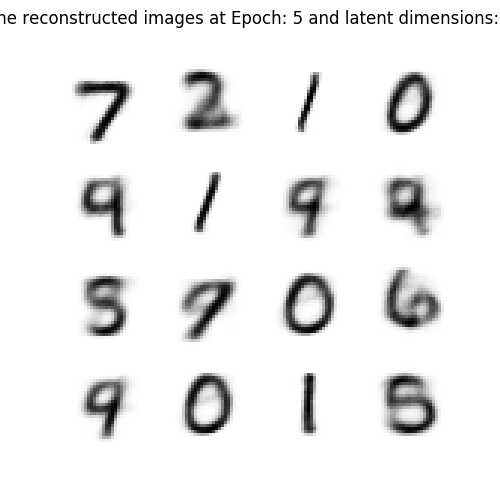
\includegraphics[width=0.23\textwidth]{../plots/task3/reconstructed_epochs5_latent2.png} & 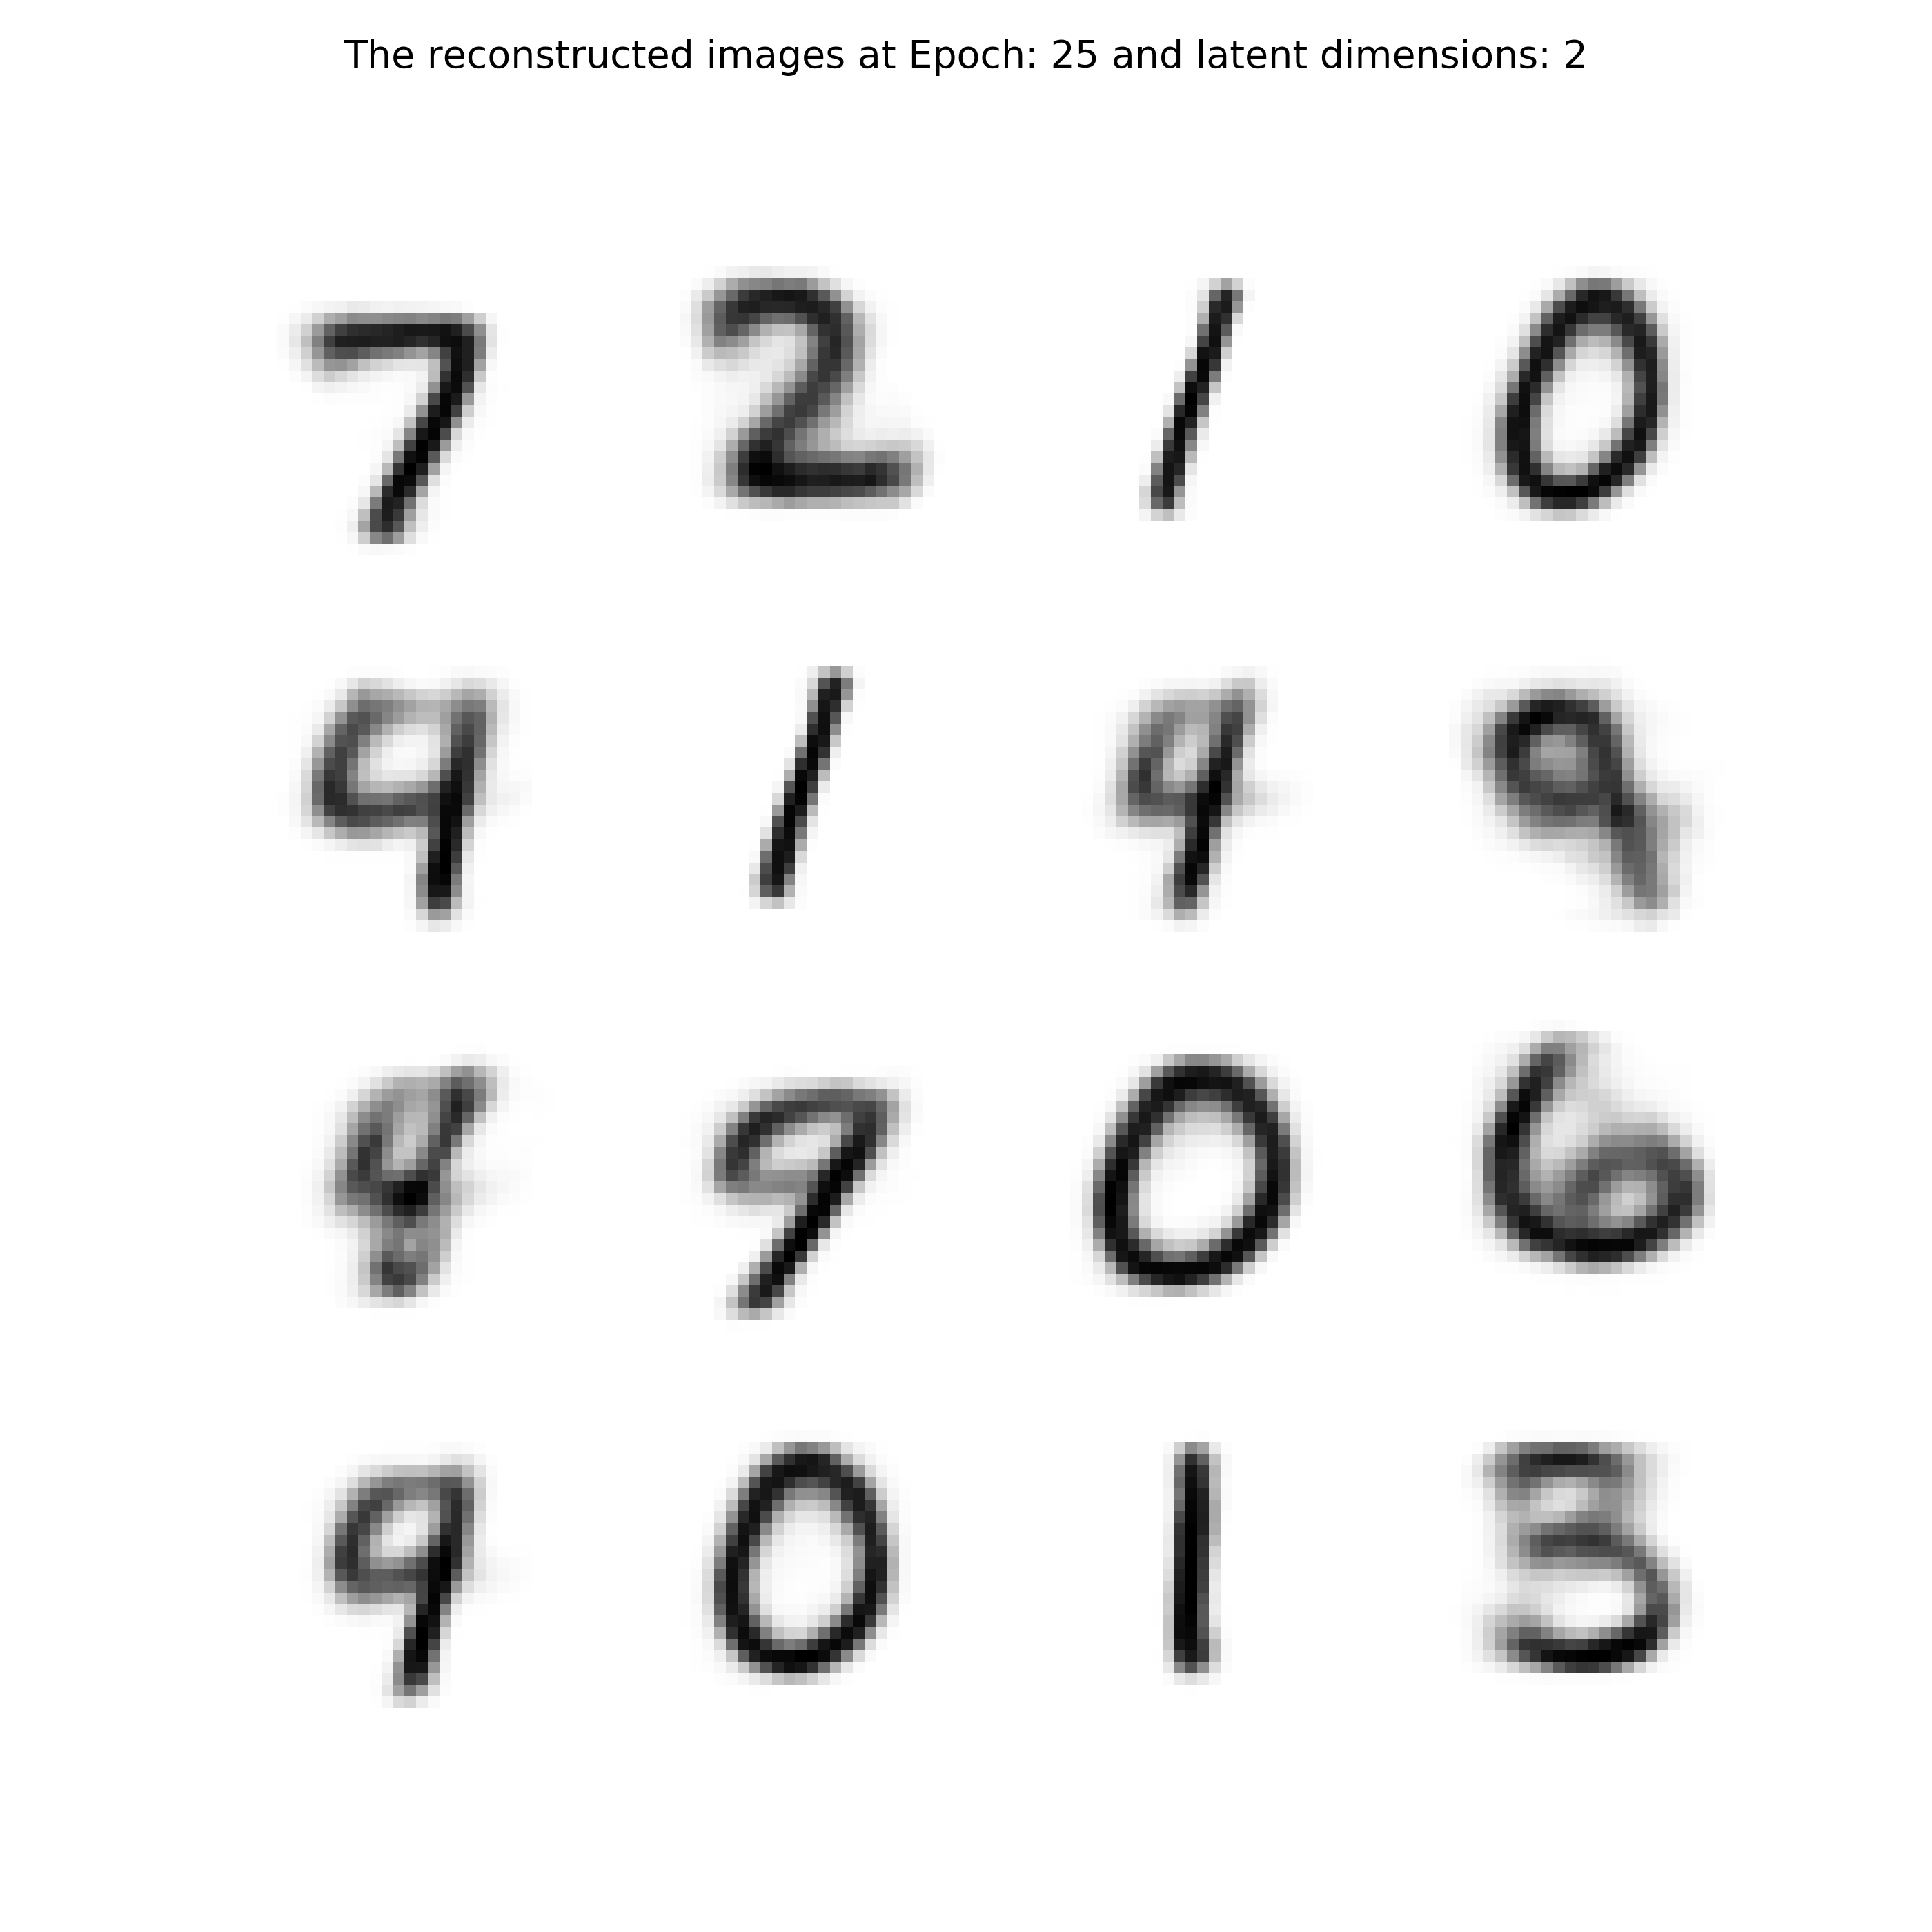
\includegraphics[width=0.23\textwidth]{../plots/task3/reconstructed_epochs25_latent2.png} &   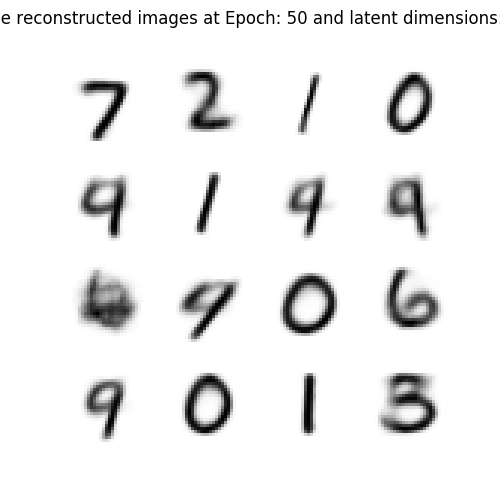
\includegraphics[width=0.23\textwidth]{../plots/task3/reconstructed_epochs50_latent2.png} \\
        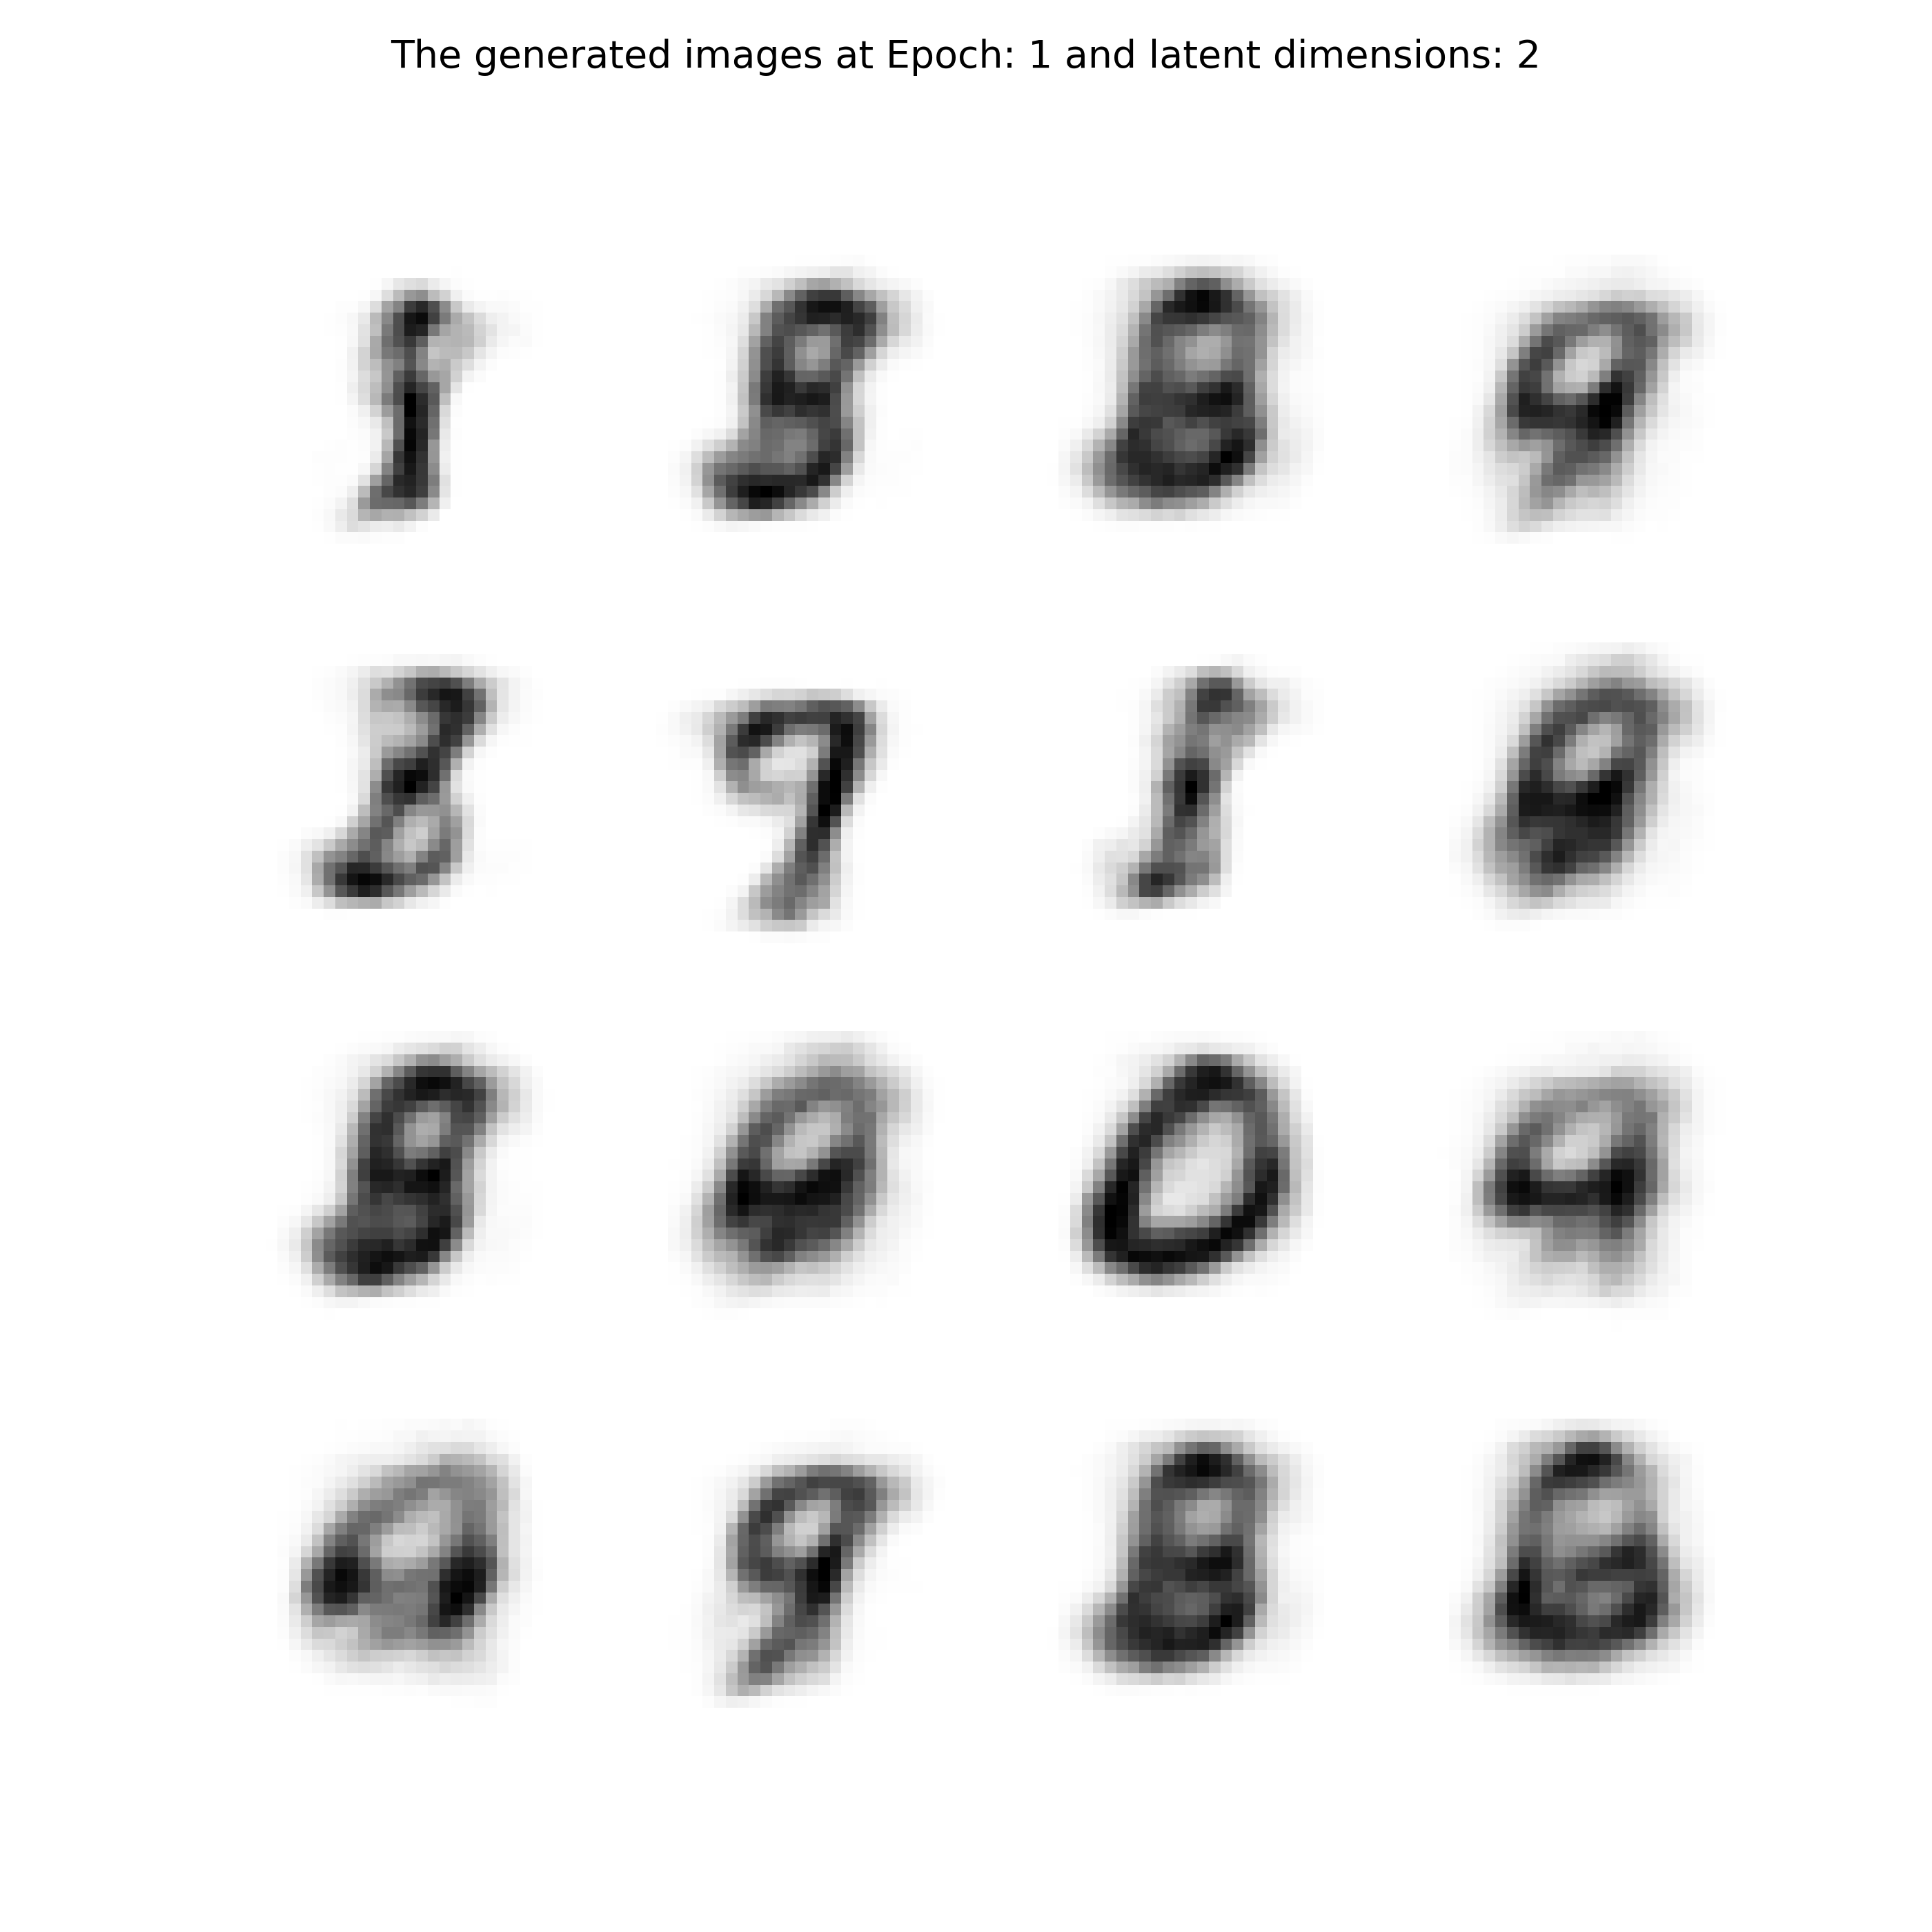
\includegraphics[width=0.23\textwidth]{../plots/task3/generated_epochs1_latent2.png} &   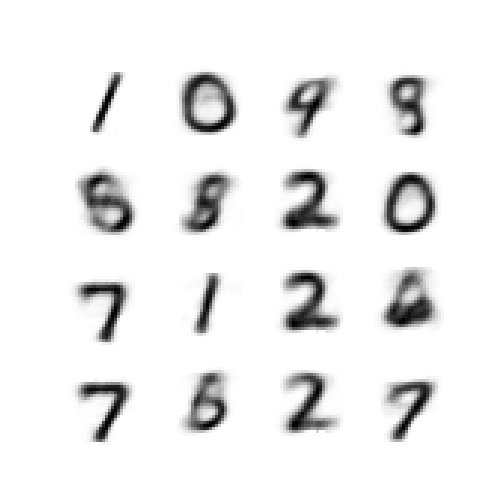
\includegraphics[width=0.23\textwidth]{../plots/task3/generated_epochs5_latent2.png} & 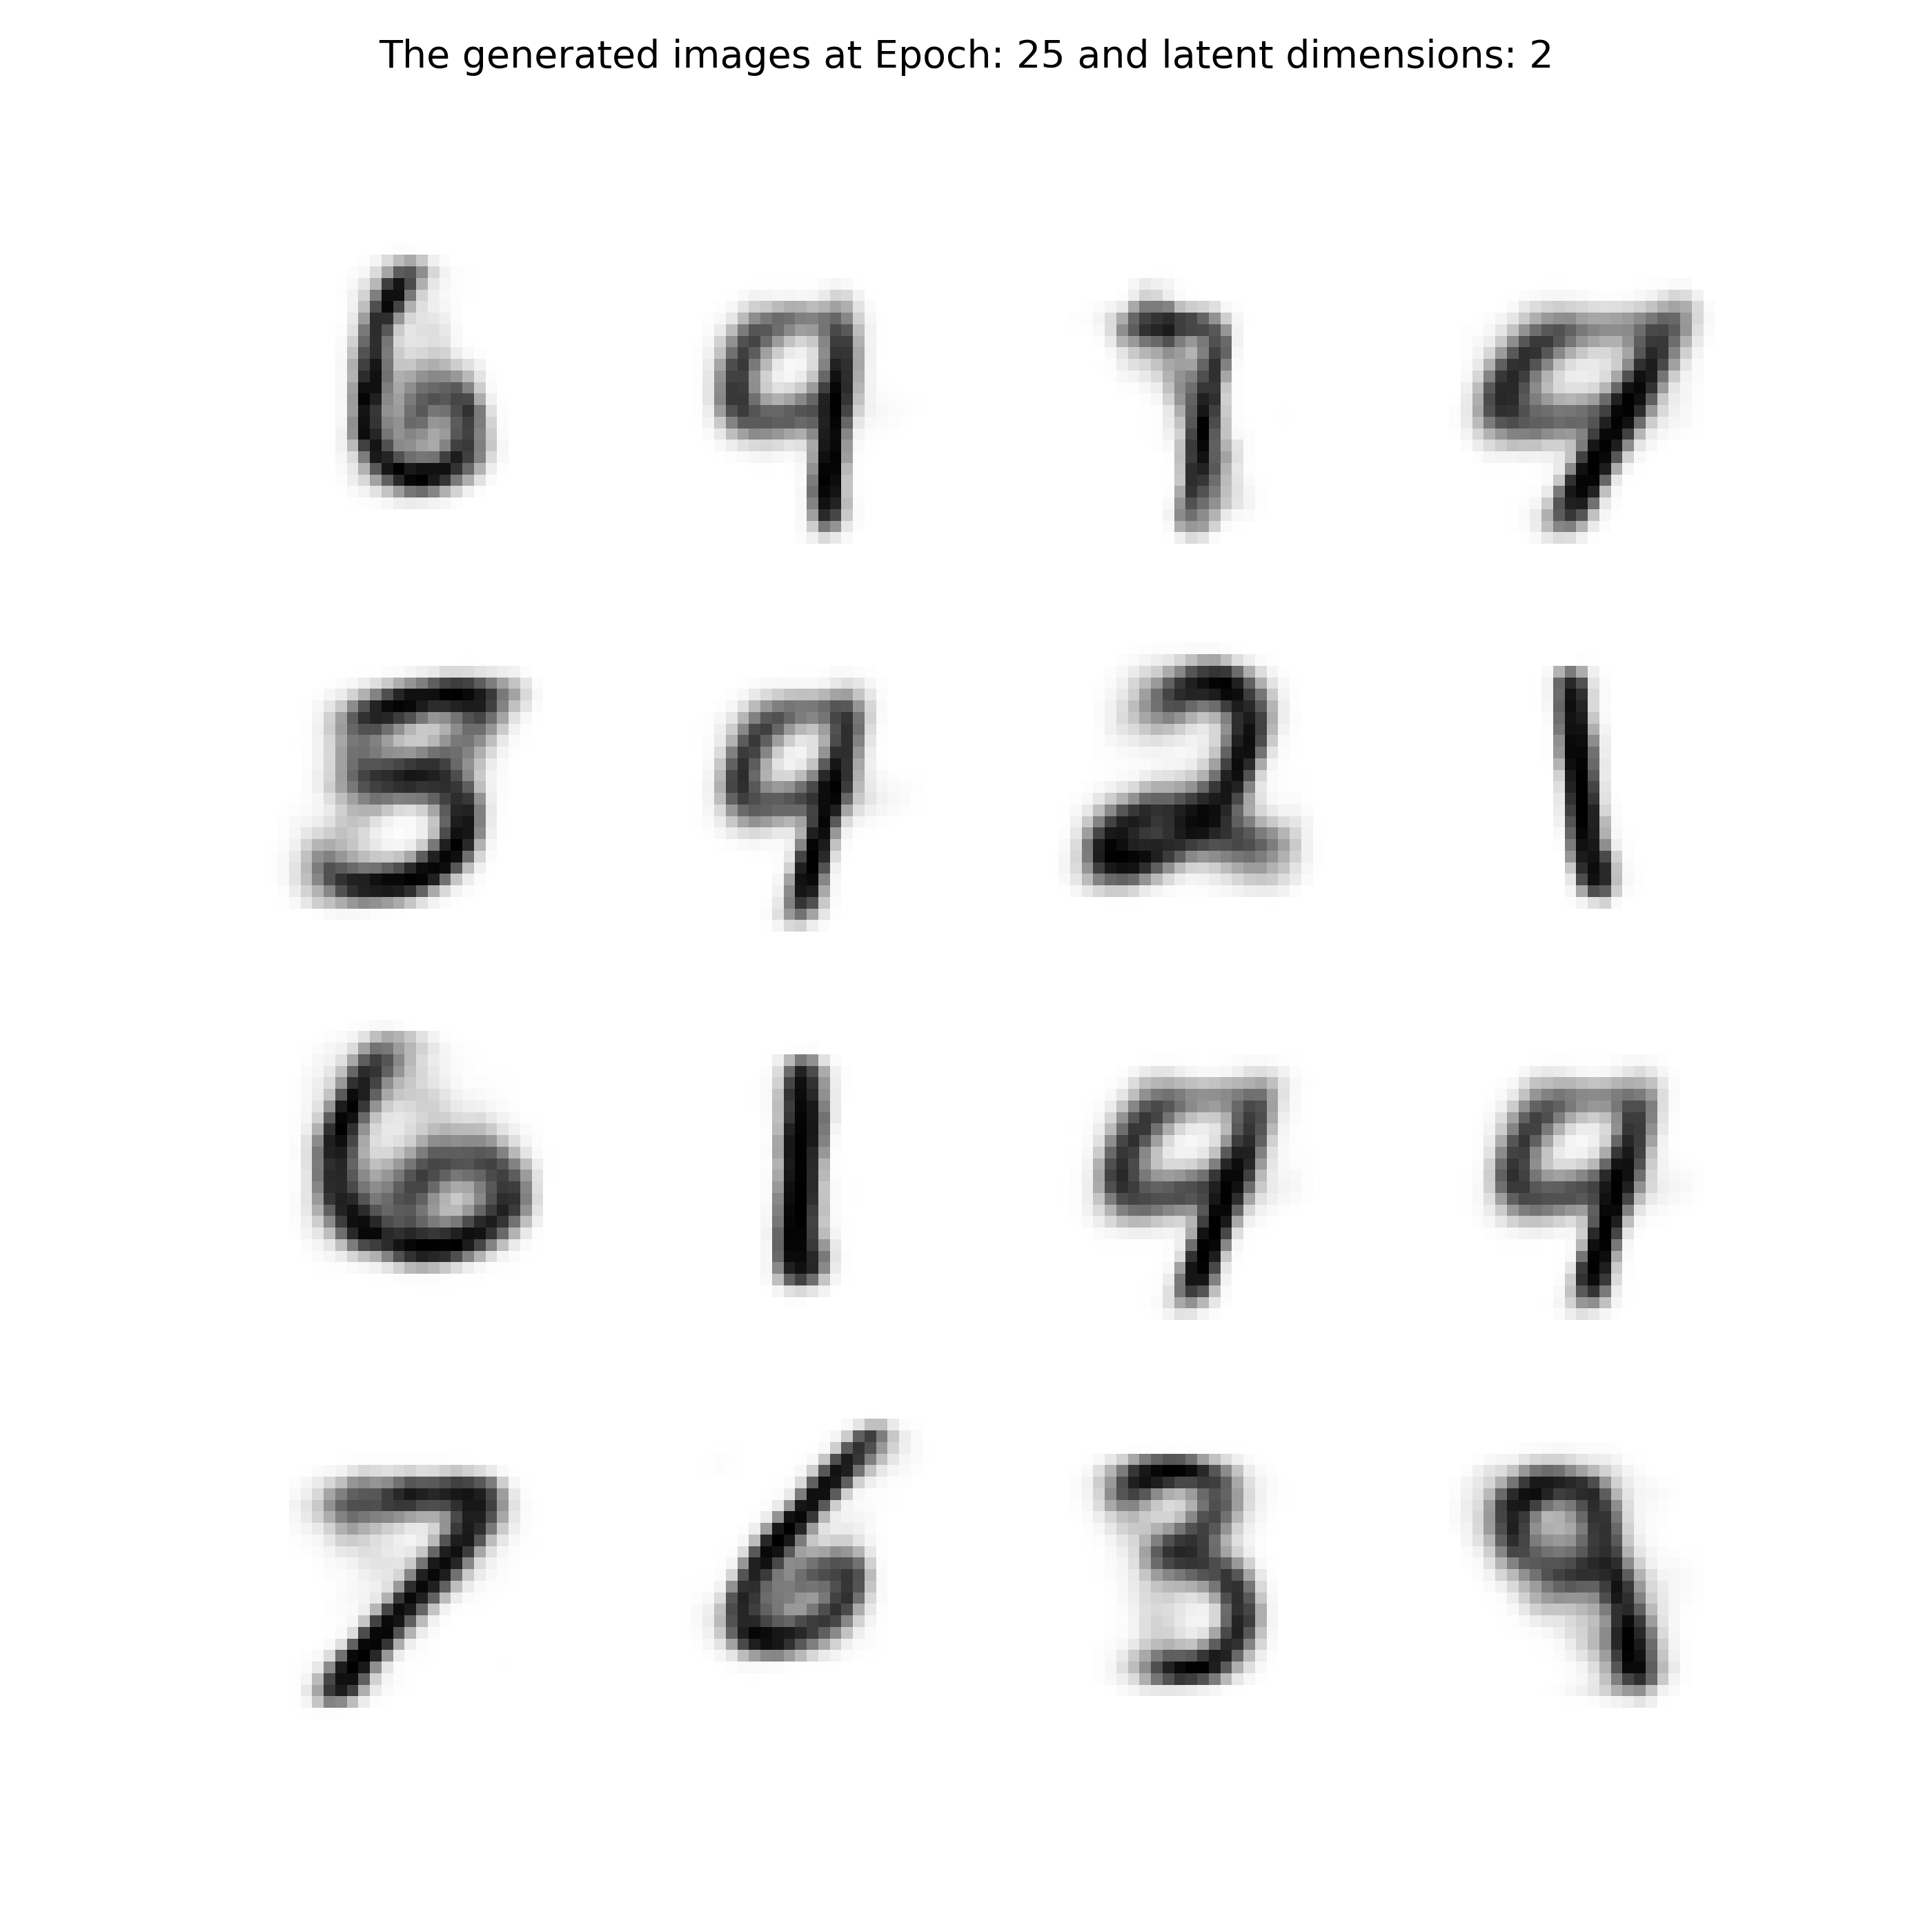
\includegraphics[width=0.23\textwidth]{../plots/task3/generated_epochs25_latent2.png} &   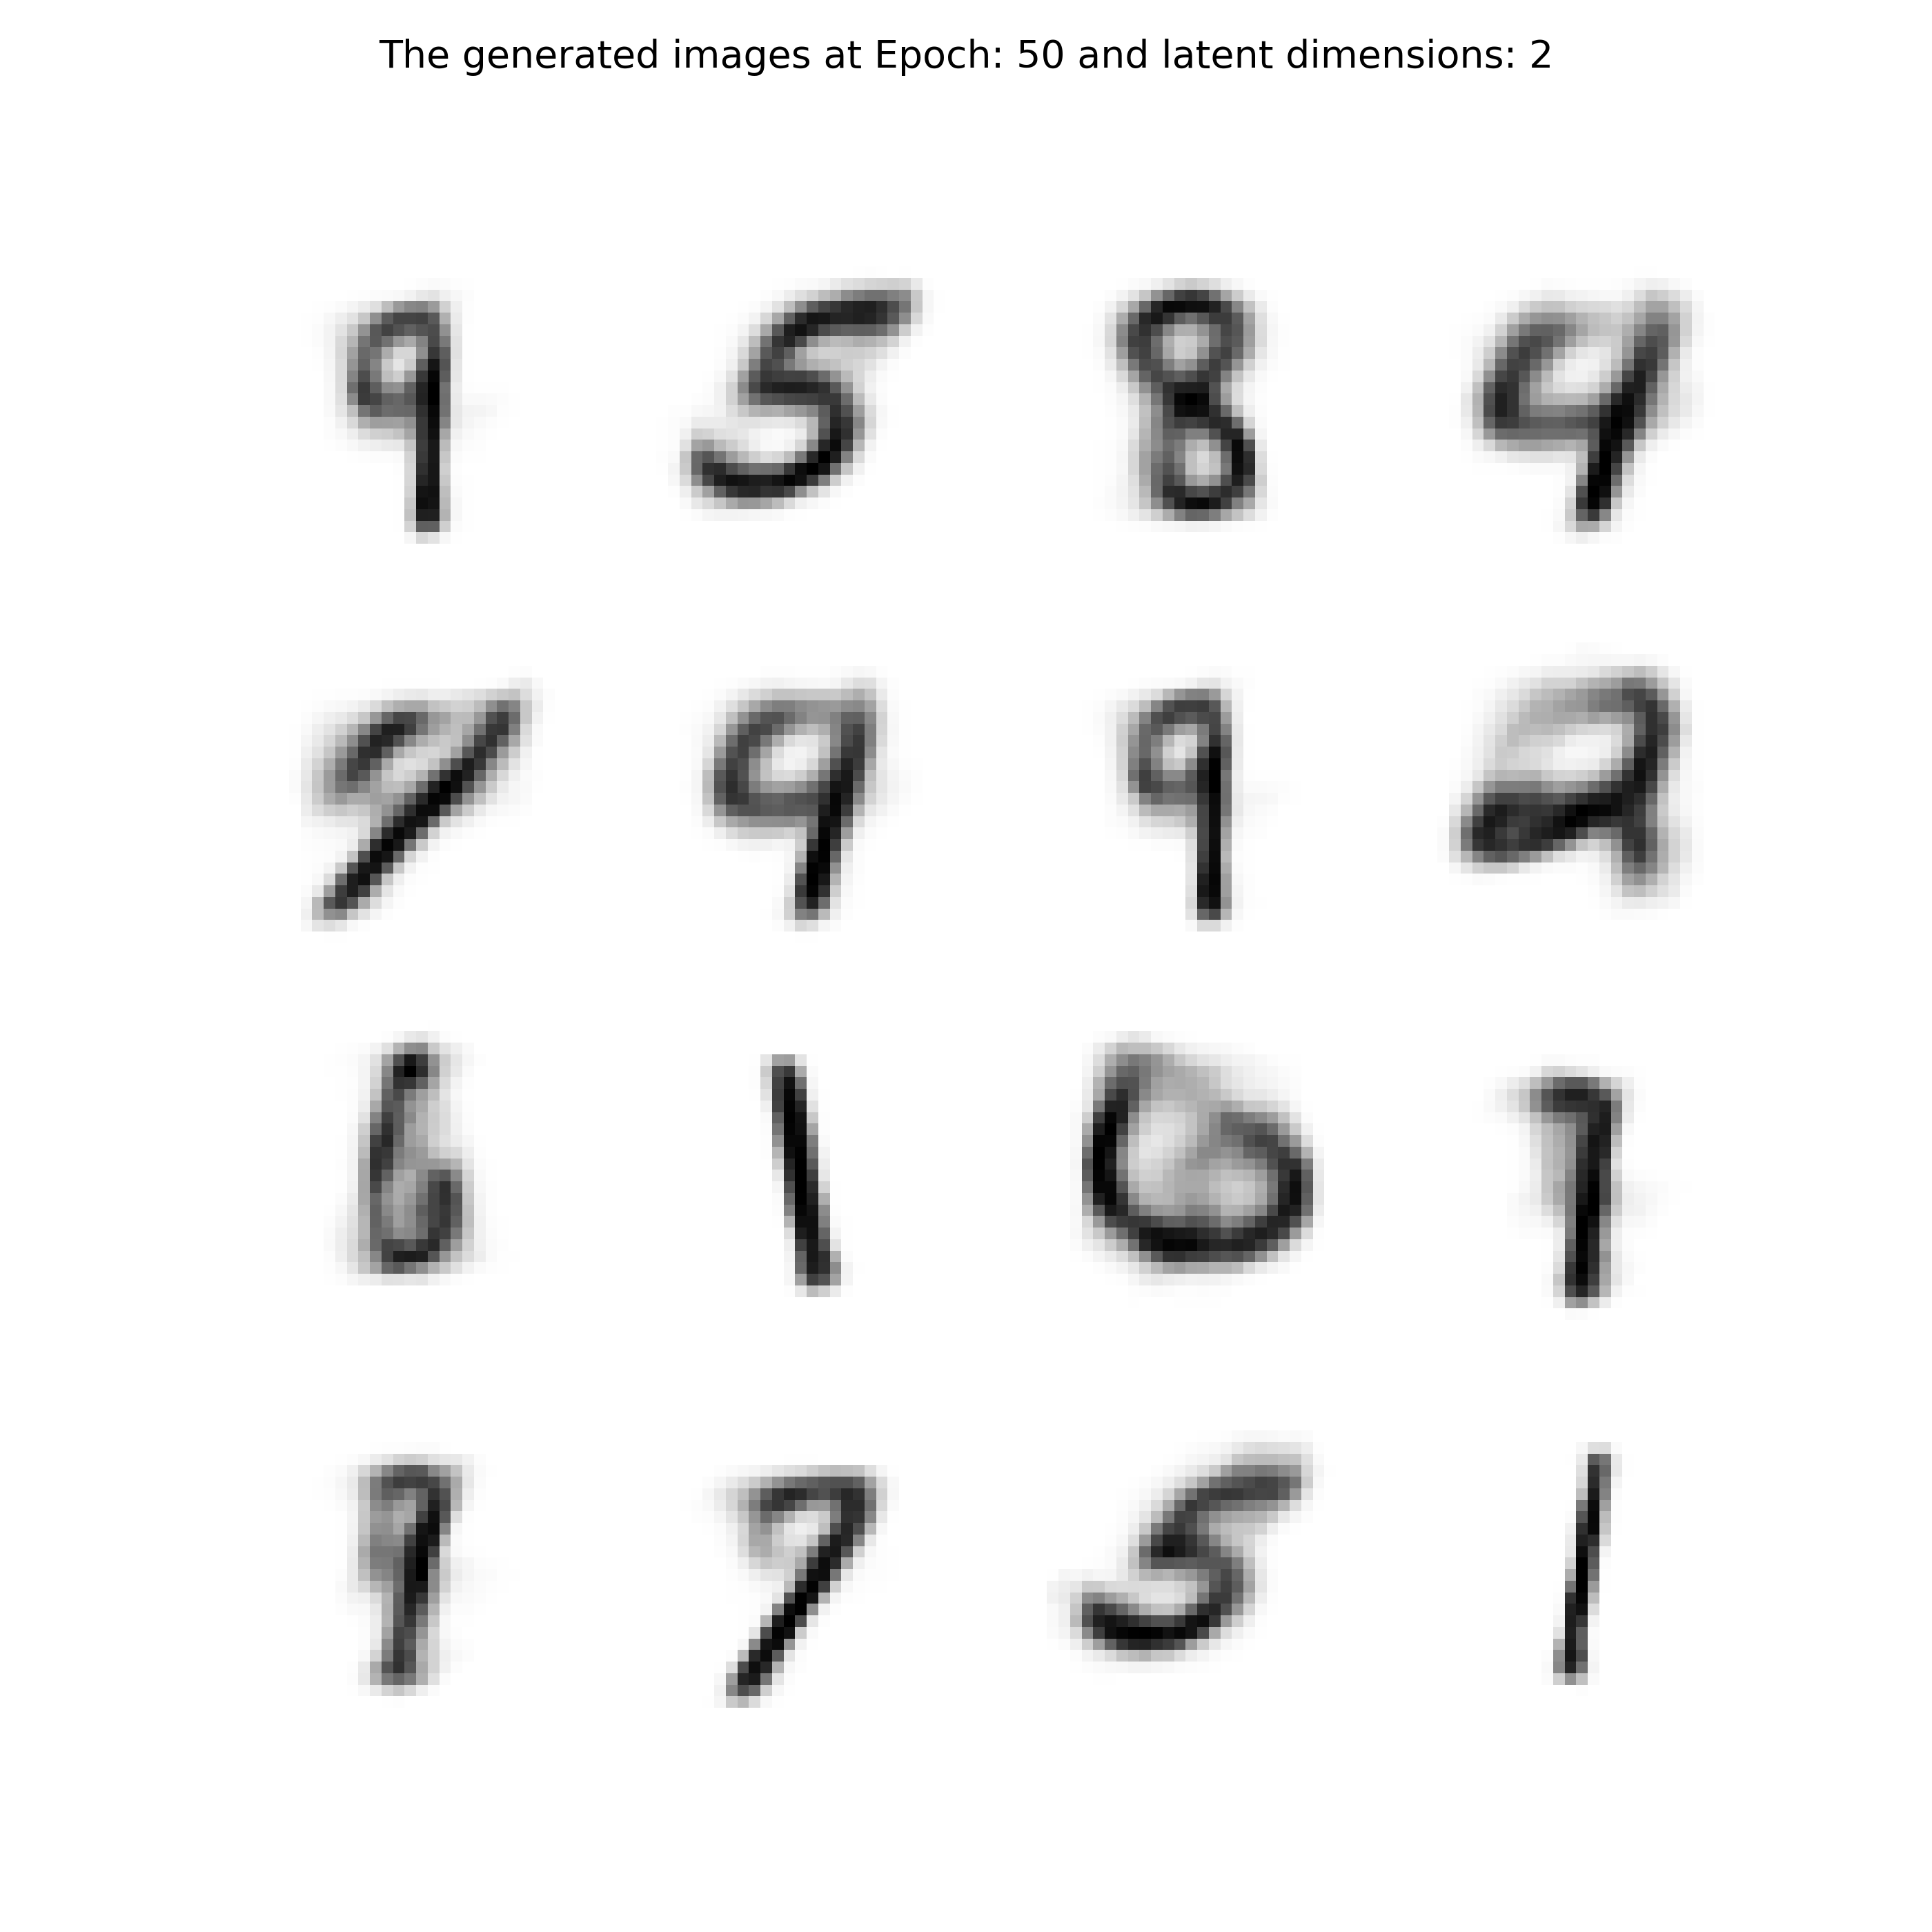
\includegraphics[width=0.23\textwidth]{../plots/task3/generated_epochs50_latent2.png} \\
\end{tabular}
\end{figure}

	\item As the VAE is trained for more epochs, the loss decreases. [\ref{fig:loss-latent-2}]
	\begin{figure}[H]
		\caption{ELBO loss}
		\label{fig:loss-latent-2}
		\centering
		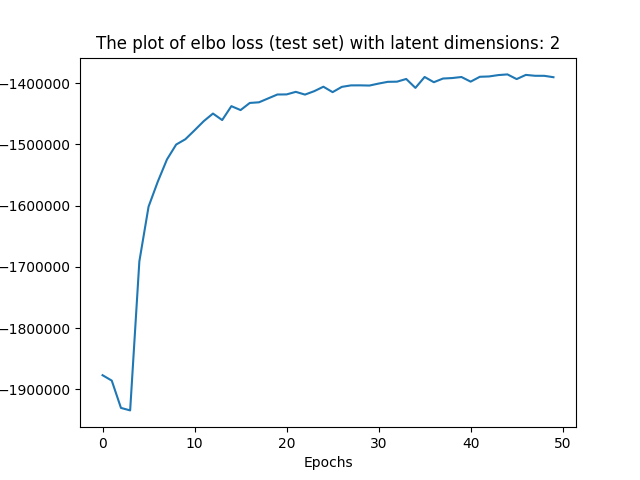
\includegraphics[width=0.45\textwidth]{../plots/task3/loss_elbo_latent2.png}
	\end{figure}	

	\item While initializing the VAE model class object, a configuration dictionary can be sent as an argument to the init function, to dynamically change the model. There are a number of configurations that can be set using the dictionary. [\ref{tab:configs_options}].
	
\begin {table}[H]
\caption {The VAE class initialization arguments} \label{tab:configs_options} 
\begin{center}
\begin{tabular}{ | m{10em} | m{20em}| } 
\hline
Argument & Description \\ 
\hline \hline
latent\_vector\_size & The dimensions of the latent vector \\ 
\hline
print\_output & Print the output plots (True or False) \\
\hline
batch\_size & Batch Size to be used \\
\hline
learning\_rate & Learning rate \\
\hline
epochs & Number of epochs\\
\hline
train\_dataloader & Pytorch dataloader for training set \\
\hline
test\_dataloader & Pytorch dataloader for test set \\
\hline
dataset\_dims & The dimensions of the dataset \\
\hline
mode & The dataset mode (mnist or mi) \\
\hline
test\_count & The number of test set data points \\
\hline
\end{tabular}
\end{center}
\end{table}

The mnist images generated using 32 dimensional latent space are more sharper. [\ref{fig:latent-32}]. The loss in this decreases more rapidly and within 50 epochs, the total loss per epoch reaches a lower value compared to the VAE trained with 2 dimensional latent space. [\ref{fig:loss-latent-32}]

\begin{figure}[H]
\caption{results obtained with a 32 dimensional latent space}
\label{fig:latent-32} 
\begin{tabular}{cccc}
	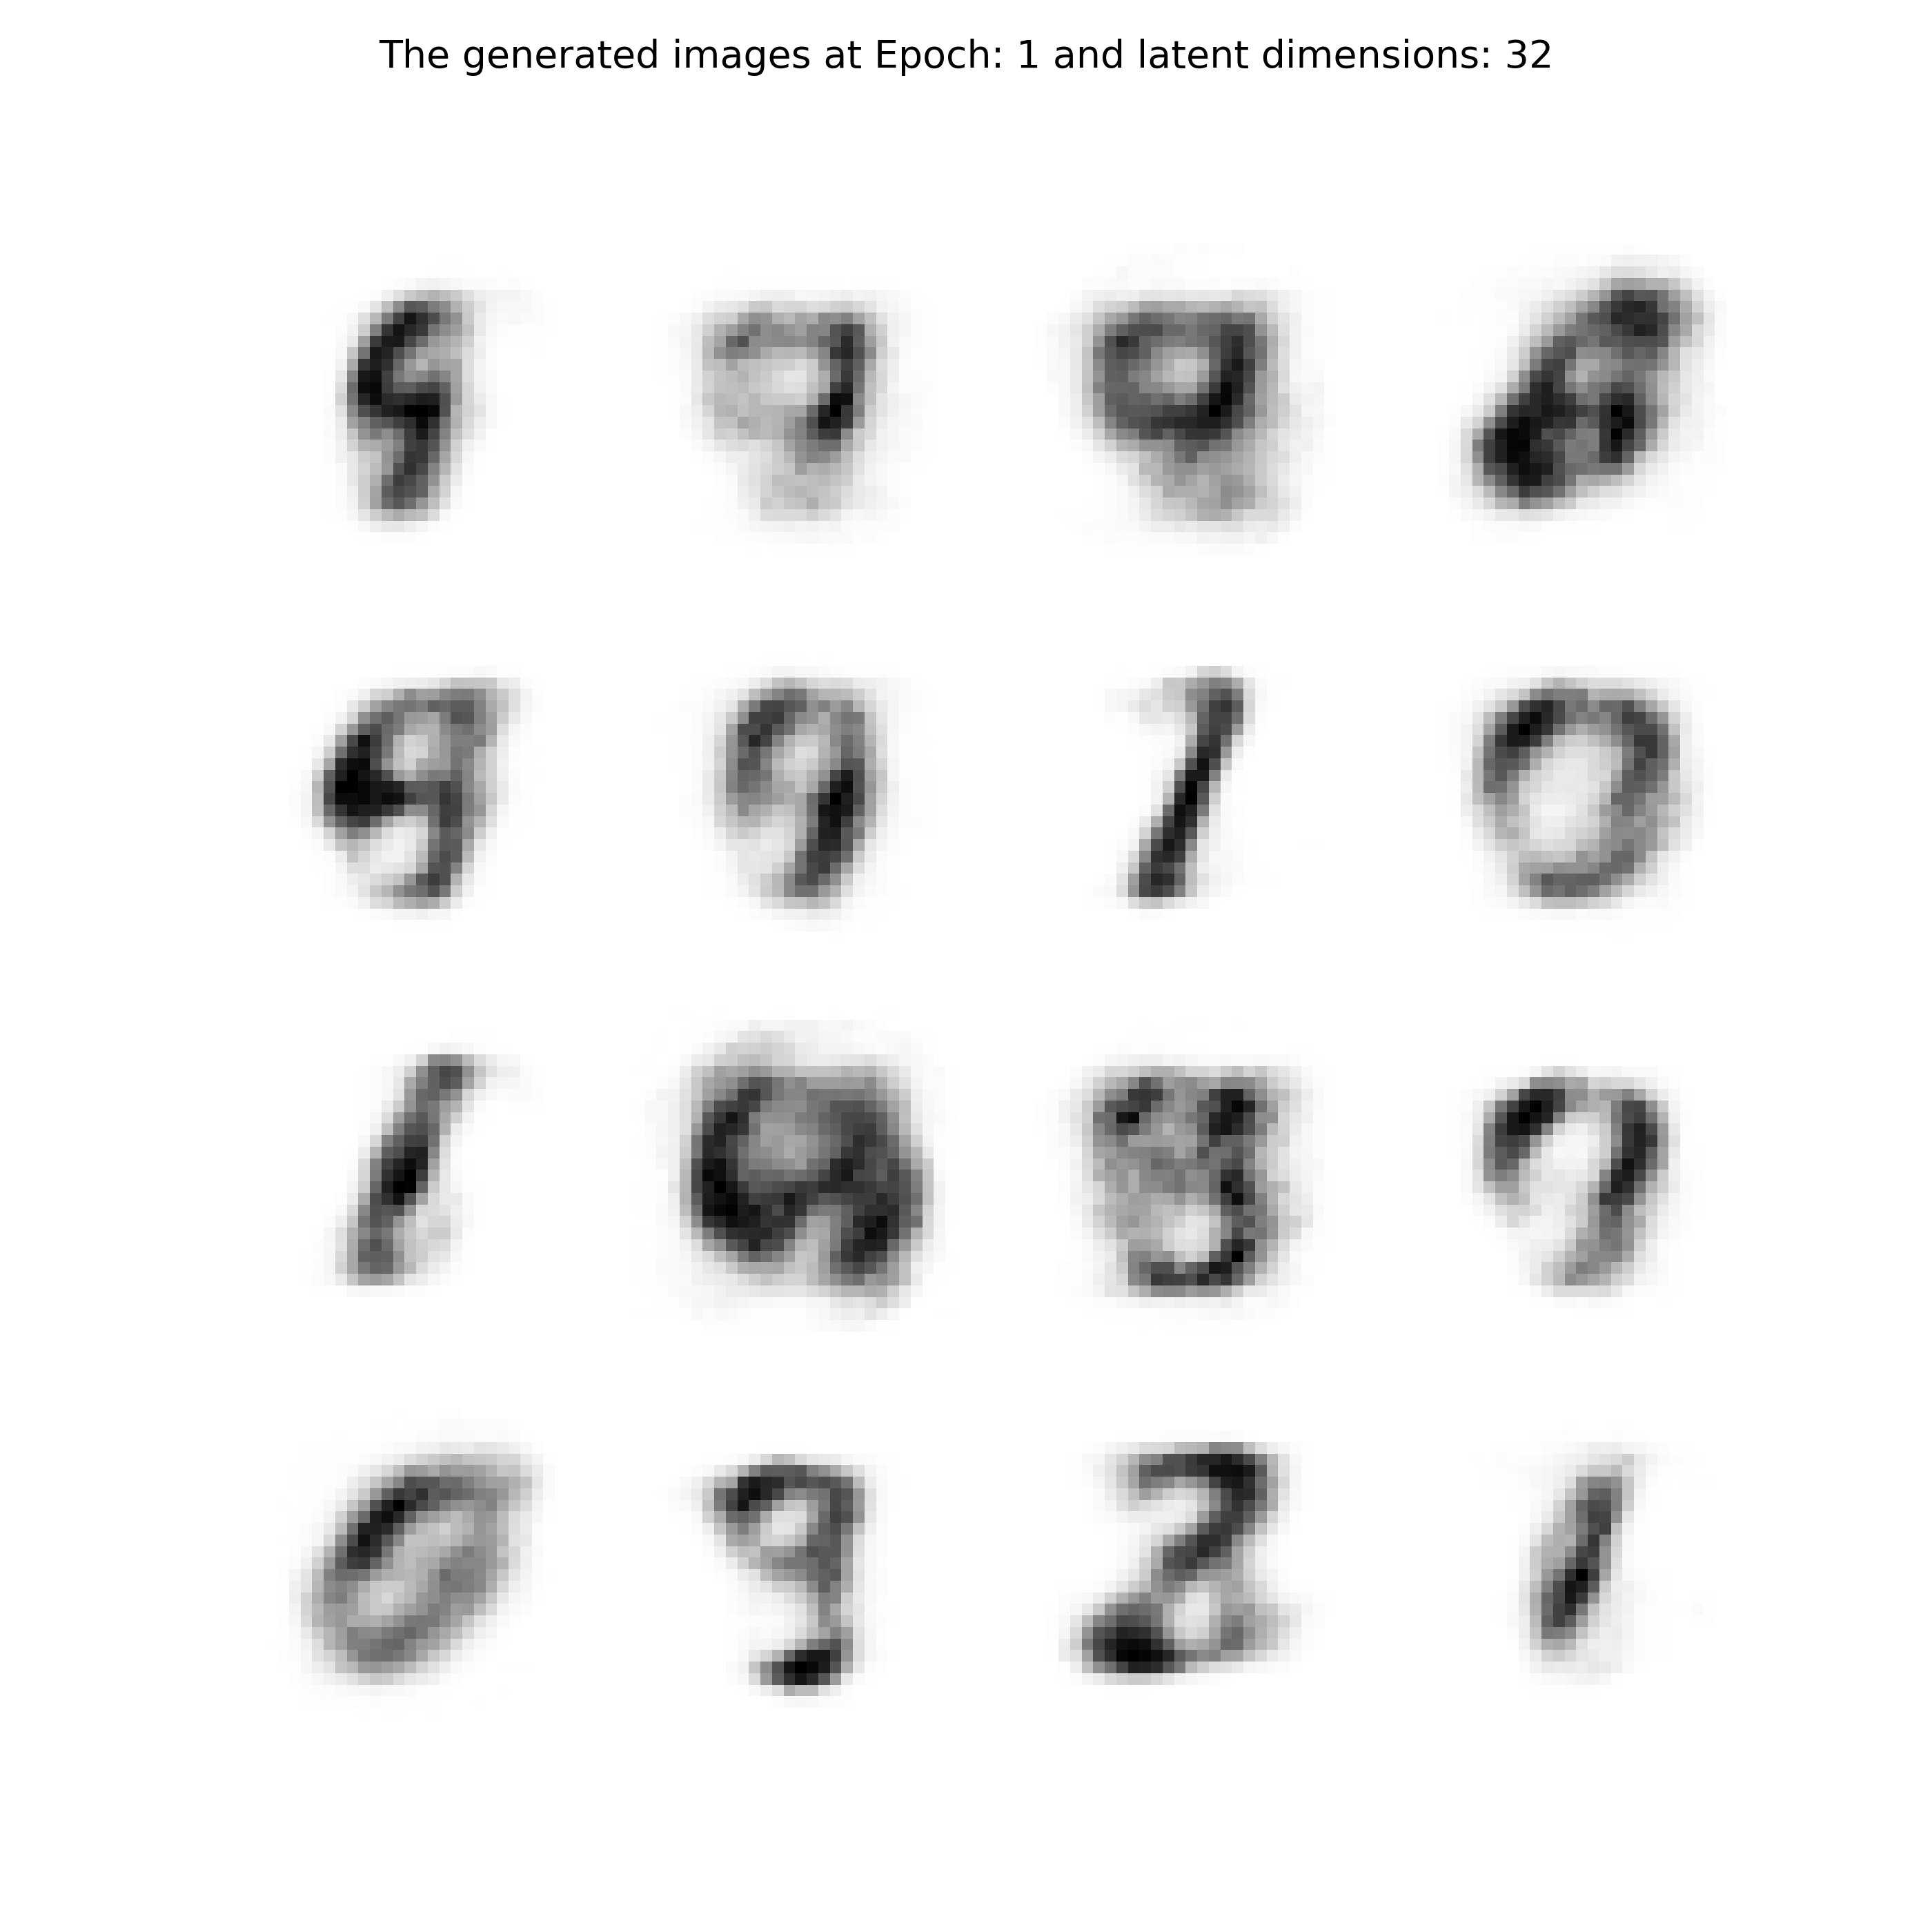
\includegraphics[width=0.23\textwidth]{../plots/task3/generated_epochs1_latent32.png} &   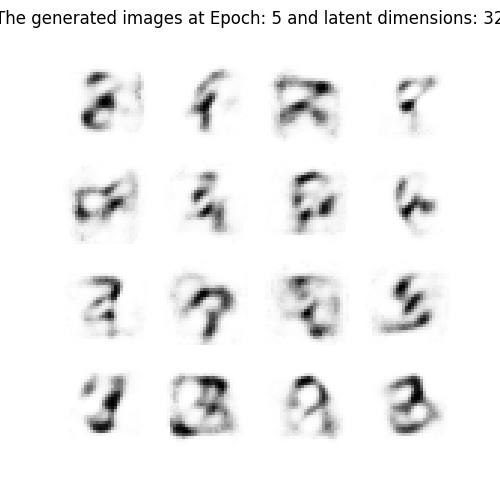
\includegraphics[width=0.23\textwidth]{../plots/task3/generated_epochs5_latent32.png} & 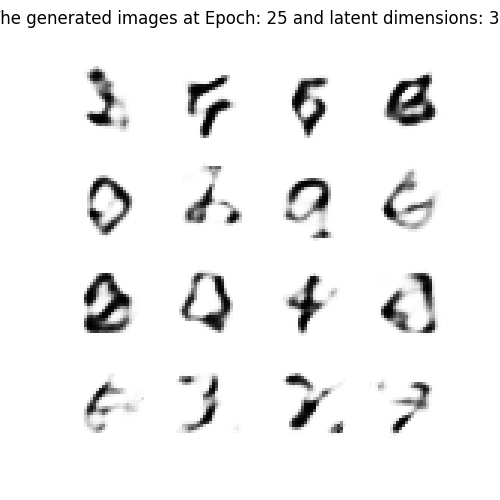
\includegraphics[width=0.23\textwidth]{../plots/task3/generated_epochs25_latent32.png} &   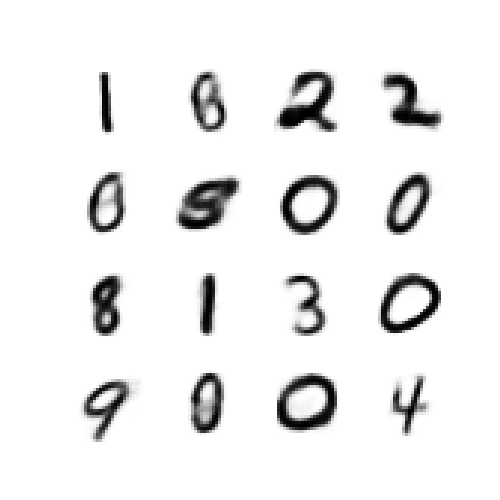
\includegraphics[width=0.23\textwidth]{../plots/task3/generated_epochs50_latent32.png} \\
\end{tabular}
\end{figure}

	\begin{figure}[H]
		\caption{ELBO loss}
		\label{fig:loss-latent-32}
		\centering
		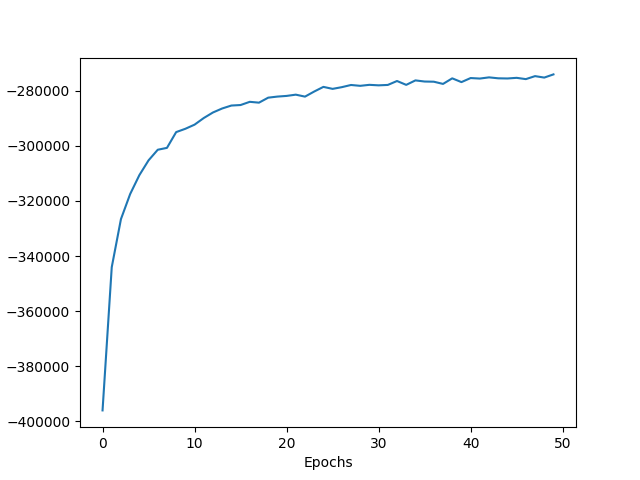
\includegraphics[width=0.45\textwidth]{../plots/task3/loss_elbo_latent32.png}
	\end{figure}

\end{enumerate}
	
\end{task}
\begin{task}{4, Fire Evacuation Planning for the MI Building}
\begin{enumerate}
	\item The training and test datasets reflect the positions of the students and employees in the campus hallways.
\begin{figure}[H]
\caption{The scatter plot of the training and test sets}
\label{fig:training-test-set} 
\begin{tabular}{cc}
	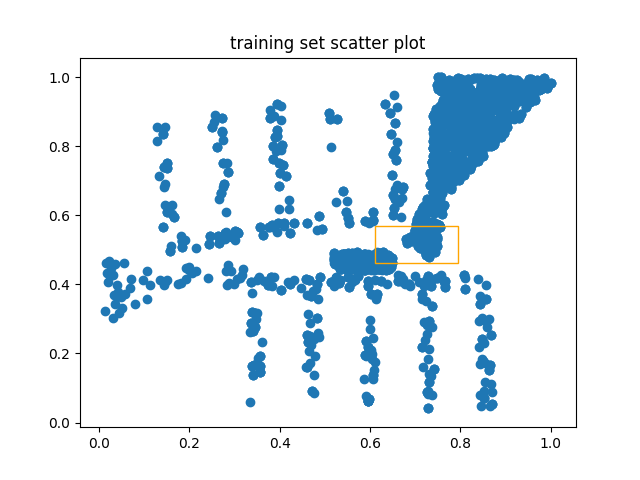
\includegraphics[width=0.45\textwidth]{../plots/task4/training_set_scatter.png} &   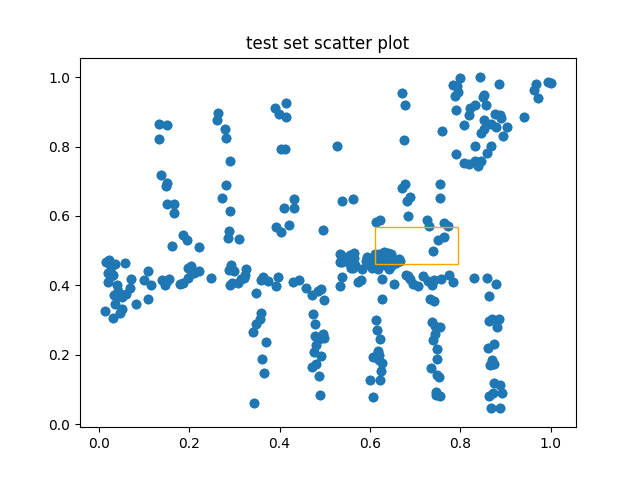
\includegraphics[width=0.45\textwidth]{../plots/task4/test_set_scatter.png} 
\end{tabular}
\end{figure}
	\item The same VAE implementation is used for training a VAE on the FireEvac data. The 'mode' argument is set to mi and the 'dataset\_dims' argument is set to 2, as the FireEvac dataset is 2 dimensional. A number of modifications have to be made to train the FireEvac dataset:
	\begin{itemize}
		\item The VAE is trained for 1000 epochs. 
		\item The learning rate of the adam optimizer is set to 0.0001 because the higher learning rate of 0.001 used in the previous task proves to be too high for training the FireEvac data. It results in a jittery model training.
		\item Mean Squared Error is used for calculating the reconstruction loss. The predicted data is the output of the decoder and the target is the input data.
		\item Relu activation function is used for the last layer of decoder, as the FireEvac data consists of positive unbounded coordinates.
	\end{itemize}
	
	\item The distribution of the data reconstructed from test set, is similar to test set distribution. [\ref{fig:reconstructed-data}]
	\begin{figure}[H]
		\caption{ELBO loss}
		\label{fig:reconstructed-data}
		\centering
		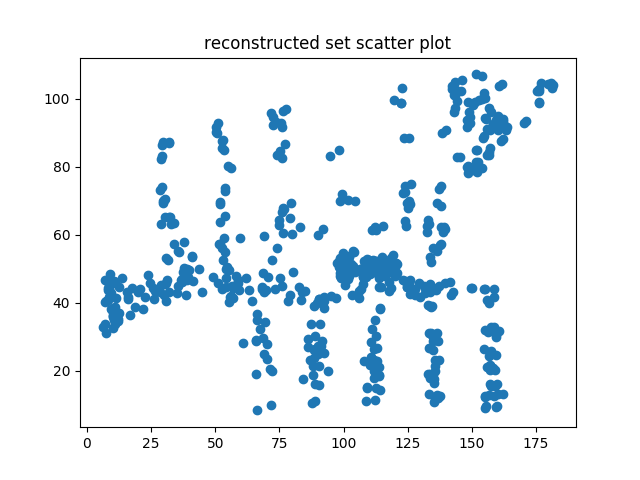
\includegraphics[width=0.45\textwidth]{../plots/task4/reconstructed_set_scatter.png}
	\end{figure}
\end{enumerate}
\end{task}
\end{document}
